% ==============================================================================
% INSTITUTO POLITÉCNICO NACIONAL
% UNIDAD PROFESIONAL INTERDISCIPLINARIA DE INGENIERÍA CAMPUS ZACATECAS (UPIIZ)
% PROGRAMA ACADÉMICO DE INGENIERÍA MECATRÓNICA
% ==============================================================================
% PLANTILLA INSTITUCIONAL DE TRABAJO TERMINAL
% Compatible con: Protocolo, Trabajo Terminal I y Trabajo Terminal II (Reporte Final)
% Motor de compilación oficial: LuaLaTeX (vía latexmk)
%
% Autores de la plantilla:
% - M. en C. Rafael Reveles Martínez
% - M. en C. Flabio Darío Mirelez Delgado
% - M. en C. Umanel Azazael Hernández González
% ==============================================================================

\documentclass[12pt,letterpaper,oneside]{report}

% ------------------------------------------------------------------------------
% CARGA DE CONFIGURACIONES MODULARES
% ------------------------------------------------------------------------------
% 1. Formato institucional, paquetes y tipografía Arial (NO MODIFICAR)
% ==============================================================================
% Plantilla Institucional de Trabajo Terminal — UPIIZ IPN
% Archivo: config/formato.tex
% ==============================================================================
% Configuración de paquetes, tipografía Arial, geometría, interlineado y formato
% normativo institucional. NO MODIFICAR SALVO INDICACIÓN DOCENTE.
% ==============================================================================

% ------------------------------------------------------------------------------
% 1. IDIOMA Y CARACTERES
% ------------------------------------------------------------------------------
\usepackage[spanish,es-tabla,es-noshorthands]{babel}
\usepackage{csquotes}
% Desactivar interferencias de babel-spanish con porcentajes en tablas
\AtBeginDocument{%
  \renewcommand{\%}{\char`\%}%
}

% ------------------------------------------------------------------------------
% 2. TIPOGRAFÍA INSTITUCIONAL: ARIAL
% ------------------------------------------------------------------------------
% Requisito institucional UPIIZ-IPN:
% - Títulos: Arial 16 pt, negrita
% - Subtítulos: Arial 14 pt, negrita
% - Cuerpo de texto: Arial 12 pt
% - Tablas y Figuras: Arial 10 pt
\usepackage{fontspec}

\IfFontExistsTF{Arial}{%
    \setmainfont{Arial}
}{%
    \IfFontExistsTF{Liberation Sans}{%
        \setmainfont{Liberation Sans}
        \typeout{AVISO: Arial no encontrada en el sistema. Usando Liberation Sans.}
    }{%
        \setmainfont{TeX Gyre Heros}
        \typeout{AVISO: Arial no encontrada. Usando TeX Gyre Heros.}
    }
}

% ------------------------------------------------------------------------------
% 3. MÁRGENES Y GEOMETRÍA DE PÁGINA
% ------------------------------------------------------------------------------
% Requisito institucional:
% - Superior: 2.5 cm
% - Inferior: 2.5 cm
% - Derecho: 2.5 cm
% - Izquierdo: 3.0 cm (encuadernación)
\usepackage{geometry}
\geometry{
    letterpaper,
    top=2.5cm,
    bottom=2.5cm,
    right=2.5cm,
    left=3.0cm,
    headheight=15pt,
    headsep=12pt,
    footskip=20pt
}

% ------------------------------------------------------------------------------
% 4. INTERLINEADO Y JUSTIFICACIÓN
% ------------------------------------------------------------------------------
% Requisito institucional: Interlineado 1.5 y texto justificado.
\usepackage{setspace}
\setstretch{1.5}
\setlength{\parindent}{1.0cm}
\setlength{\parskip}{0pt}

% ------------------------------------------------------------------------------
% 5. FORMATO DE TÍTULOS Y SUBTÍTULOS (titlesec)
% ------------------------------------------------------------------------------
\usepackage{titlesec}

% Títulos de Capítulos: Arial 16 pt, negrita
\titleformat{\chapter}[hang]
    {\fontsize{16}{20}\bfseries\sffamily}
    {\thechapter.\ }
    {0pt}
    {\fontsize{16}{20}\bfseries\sffamily}

\titlespacing*{\chapter}{0pt}{-10pt}{15pt}

% Títulos de Secciones (Subtítulos): Arial 14 pt, negrita
\titleformat{\section}
    {\fontsize{14}{18}\bfseries\sffamily}
    {\thesection\ }
    {0pt}
    {\fontsize{14}{18}\bfseries\sffamily}

\titlespacing*{\section}{0pt}{12pt}{6pt}

% Títulos de Subsecciones: Arial 12 pt, negrita
\titleformat{\subsection}
    {\fontsize{12}{15}\bfseries\sffamily}
    {\thesubsection\ }
    {0pt}
    {\fontsize{12}{15}\bfseries\sffamily}

\titlespacing*{\subsection}{0pt}{10pt}{4pt}

% Títulos de Sub-subsecciones: Arial 12 pt
\titleformat{\subsubsection}
    {\fontsize{12}{15}\itshape\sffamily}
    {\thesubsubsection\ }
    {0pt}
    {\fontsize{12}{15}\itshape\sffamily}

\titlespacing*{\subsubsection}{0pt}{8pt}{3pt}

% ------------------------------------------------------------------------------
% 6. FORMATO DE TABLAS Y FIGURAS
% ------------------------------------------------------------------------------
% Requisito institucional: Arial 10 pt para pies de figura y encabezados de tabla.
\usepackage{caption}
\captionsetup{
    font={small},           % 10 pt
    labelfont={bf,small},   % Etiqueta en negrita
    labelsep=period,        % Punto tras el número: "Figura 1.1."
    format=hang,
    justification=justified
}

\usepackage{subcaption}
\usepackage{booktabs}
\usepackage{tabularx}
\usepackage{longtable}
\usepackage{multirow}
\usepackage{array}
\usepackage{float}
\usepackage{graphicx}
\usepackage{pdfpages}

% ------------------------------------------------------------------------------
% 7. MATEMÁTICAS Y UNIDADES FÍSICAS
% ------------------------------------------------------------------------------
\usepackage{amsmath}
\usepackage{amssymb}
\usepackage{amsfonts}
\usepackage{mathtools}
\usepackage{siunitx}
\sisetup{
    output-decimal-marker = {.},
    per-mode = symbol,
    range-phrase = { a },
    range-units = single
}

% ------------------------------------------------------------------------------
% 8. LISTAS Y ENUMERACIONES
% ------------------------------------------------------------------------------
\usepackage{enumitem}
\setlist{leftmargin=1.5cm, noitemsep, topsep=4pt}

% ------------------------------------------------------------------------------
% 9. ENCABEZADOS Y PIES DE PÁGINA (fancyhdr)
% ------------------------------------------------------------------------------
\usepackage{fancyhdr}
\pagestyle{fancy}
\fancyhf{}
\renewcommand{\headrulewidth}{0pt}
\cfoot{\thepage}

% Estilo para páginas iniciales de capítulo
\fancypagestyle{plain}{%
    \fancyhf{}
    \cfoot{\thepage}
    \renewcommand{\headrulewidth}{0pt}
}

% ------------------------------------------------------------------------------
% 10. HIPERVÍNCULOS Y METADATOS PDF
% ------------------------------------------------------------------------------
\usepackage[
    colorlinks=true,
    linkcolor=black,
    citecolor=black,
    urlcolor=black,
    bookmarks=true,
    bookmarksnumbered=true,
    pdfdisplaydoctitle=true,
    hidelinks
]{hyperref}
\usepackage{bookmark}

% ------------------------------------------------------------------------------
% 11. CÓDIGO FUENTE (listings)
% ------------------------------------------------------------------------------
\usepackage{listings}
\usepackage{xcolor}

\definecolor{codegreen}{rgb}{0,0.6,0}
\definecolor{codegray}{rgb}{0.5,0.5,0.5}
\definecolor{codepurple}{rgb}{0.58,0,0.82}
\definecolor{backcolour}{rgb}{0.97,0.97,0.97}

\lstdefinestyle{estilocodigo}{
    backgroundcolor=\color{backcolour},
    commentstyle=\color{codegreen},
    keywordstyle=\color{blue}\bfseries,
    numberstyle=\tiny\color{codegray},
    stringstyle=\color{codepurple},
    basicstyle=\ttfamily\fontsize{9}{11}\selectfont,
    breakatwhitespace=false,
    breaklines=true,
    captionpos=b,
    keepspaces=true,
    numbers=left,
    numbersep=5pt,
    showspaces=false,
    showstringspaces=false,
    showtabs=false,
    tabsize=2,
    frame=single,
    rulecolor=\color{codegray}
}
\lstset{style=estilocodigo}


% 2. Catálogo institucional de Líneas de Trabajo (Anexo 1) (NO MODIFICAR)
% ==============================================================================
% Plantilla Institucional de Trabajo Terminal — UPIIZ IPN
% Archivo: config/lineas-trabajo.tex
% ==============================================================================
% CATÁLOGO OFICIAL DE LÍNEAS DE TRABAJO INSTITUCIONALES (ANEXO 1)
% Programa Académico de Ingeniería Mecatrónica — UPIIZ IPN
%
% Este archivo define el catálogo oficial inmutable de las 6 Líneas de Trabajo.
% El estudiante selecciona su línea mediante el comando \LineaTrabajo{...} en
% config/datos.tex sin necesidad de modificar este archivo.
% ==============================================================================

\usepackage{etoolbox}

\newif\ifLineaTrabajoValida
\LineaTrabajoValidafalse

\newcommand{\LineaTrabajo}[1]{%
  \def\NumeroLineaTrabajo{#1}%
  \ifstrequal{#1}{I}{%
    \LineaTrabajoValidatrue
    \def\NombreLineaTrabajo{Diseño e implementación de un sistema robótico, dispositivos o sistemas Mecatrónicos.}%
    \def\EntregableLineaTrabajo{Prototipo, Interfaz Hombre-Máquina.}%
    \def\DescripcionLineaTrabajo{Las 4 áreas de la Mecatrónica se desarrollan con el mismo grado de complejidad y detalle.}%
    \def\MaximoAlumnosLineaTrabajo{3}%
  }{%
  \ifstrequal{#1}{II}{%
    \LineaTrabajoValidatrue
    \def\NombreLineaTrabajo{Diseño e implementación de una máquina o mecanismo.}%
    \def\EntregableLineaTrabajo{Prototipo, Interfaz Hombre-Máquina.}%
    \def\DescripcionLineaTrabajo{Énfasis en la mecánica y menor complejidad en las demás áreas.}%
    \def\MaximoAlumnosLineaTrabajo{2}%
  }{%
  \ifstrequal{#1}{III}{%
    \LineaTrabajoValidatrue
    \def\NombreLineaTrabajo{Diseño e implementación de componentes o sistemas electrónicos.}%
    \def\EntregableLineaTrabajo{Prototipo, Interfaz Hombre-Máquina.}%
    \def\DescripcionLineaTrabajo{Énfasis en la electrónica y menor complejidad en las demás áreas.}%
    \def\MaximoAlumnosLineaTrabajo{2}%
  }{%
  \ifstrequal{#1}{IV}{%
    \LineaTrabajoValidatrue
    \def\NombreLineaTrabajo{Diseño e implementación de sistemas o técnicas de control.}%
    \def\EntregableLineaTrabajo{Prototipo, Interfaz Hombre-Máquina.}%
    \def\DescripcionLineaTrabajo{Énfasis en el control y menor complejidad en las demás áreas.}%
    \def\MaximoAlumnosLineaTrabajo{2}%
  }{%
  \ifstrequal{#1}{V}{%
    \LineaTrabajoValidatrue
    \def\NombreLineaTrabajo{Diseño y desarrollo de software para el control de sistemas o procesos.}%
    \def\EntregableLineaTrabajo{Software, Interfaz Hombre-Máquina y prototipo.}%
    \def\DescripcionLineaTrabajo{Énfasis en la programación y menor complejidad en las demás áreas.}%
    \def\MaximoAlumnosLineaTrabajo{2}%
  }{%
  \ifstrequal{#1}{VI}{%
    \LineaTrabajoValidatrue
    \def\NombreLineaTrabajo{Puesta en operación, optimización o automatización de un proceso o sistema industrial.}%
    \def\EntregableLineaTrabajo{Proceso o sistema industrial en operación.}%
    \def\DescripcionLineaTrabajo{Puesta en operación y automatización de procesos industriales.}%
    \def\MaximoAlumnosLineaTrabajo{2}%
  }{%
    \LineaTrabajoValidafalse
    \def\NombreLineaTrabajo{Línea de trabajo no válida}%
    \def\EntregableLineaTrabajo{}%
    \def\DescripcionLineaTrabajo{}%
    \def\MaximoAlumnosLineaTrabajo{0}%
    \PackageWarning{PlantillaUPIIZ}{%
      Línea de trabajo '#1' no válida. Las opciones permitidas son: I, II, III, IV, V y VI.%
    }%
  }}}}}}%
}


% 3. Macros, lógica condicional y dispatcher (NO MODIFICAR)
% ==============================================================================
% Plantilla Institucional de Trabajo Terminal — UPIIZ IPN
% Archivo: config/comandos.tex
% ==============================================================================
% Macros, lógica de selección de tipo de documento (PROTOCOLO / TTI / TTII),
% despacho de portadas, firmas dinámicas y referencias cruzadas.
% ==============================================================================

\usepackage{etoolbox}

% ------------------------------------------------------------------------------
% 1. SISTEMA CENTRALIZADO DE TIPO DE DOCUMENTO (PROTOCOLO / TTI / TTII)
% ------------------------------------------------------------------------------
% Definición de booleanos de estado global
\newif\ifProtocolo
\newif\ifTTI
\newif\ifTTII

% Macro principal de configuración
\newcommand{\TipoDocumento}[1]{%
  \edef\tipoDocParam{\detokenize{#1}}%
  \Protocolofalse
  \TTIfalse
  \TTIIfalse
  % Comparación normalizada
  \ifstrequal{#1}{PROTOCOLO}{%
    \Protocolotrue
    \def\TipoDocCodigo{PROTOCOLO}%
  }{%
  \ifstrequal{#1}{protocolo}{%
    \Protocolotrue
    \def\TipoDocCodigo{PROTOCOLO}%
  }{%
  \ifstrequal{#1}{TTI}{%
    \TTItrue
    \def\TipoDocCodigo{TTI}%
  }{%
  \ifstrequal{#1}{tti}{%
    \TTItrue
    \def\TipoDocCodigo{TTI}%
  }{%
  \ifstrequal{#1}{TT1}{%
    \TTItrue
    \def\TipoDocCodigo{TTI}%
  }{%
  \ifstrequal{#1}{TTII}{%
    \TTIItrue
    \def\TipoDocCodigo{TTII}%
  }{%
  \ifstrequal{#1}{ttii}{%
    \TTIItrue
    \def\TipoDocCodigo{TTII}%
  }{%
  \ifstrequal{#1}{TT2}{%
    \TTIItrue
    \def\TipoDocCodigo{TTII}%
  }{%
    \PackageWarning{PlantillaUPIIZ}{%
      Tipo de documento '#1' no reconocido. Opciones validas: PROTOCOLO, TTI, TTII. %
      Se usara TTI por defecto.%
    }%
    \TTItrue
    \def\TipoDocCodigo{TTI}%
  }}}}}}}}%
}

% Macros auxiliares para consulta de estado
\newcommand{\EsProtocolo}[1]{\ifProtocolo #1\fi}
\newcommand{\EsTTI}[1]{\ifTTI #1\fi}
\newcommand{\EsTTII}[1]{\ifTTII #1\fi}

% Nombres legibles para títulos y texto
\newcommand{\NombreTipoDocumento}{%
  \ifProtocolo Protocolo de Trabajo Terminal\fi%
  \ifTTI Trabajo Terminal I\fi%
  \ifTTII Trabajo Terminal II\fi%
}

\newcommand{\NombreTipoDocumentoMayusculas}{%
  \ifProtocolo PROTOCOLO DE TRABAJO TERMINAL\fi%
  \ifTTI TRABAJO TERMINAL I\fi%
  \ifTTII TRABAJO TERMINAL II\fi%
}

\newcommand{\subtituloPortada}{%
  \ifProtocolo PROTOCOLO DE TRABAJO TERMINAL\fi%
  \ifTTI REPORTE TÉCNICO DE TRABAJO TERMINAL I\fi%
  \ifTTII REPORTE FINAL DE TRABAJO TERMINAL\fi%
}

\newcommand{\tituloValidacion}{%
  \ifTTI Análisis y validación del diseño\else Análisis y validación de resultados\fi%
}

% ------------------------------------------------------------------------------
% 2. VALIDACIÓN DE CAMPOS OBLIGATORIOS (ADVERTENCIAS EN LOG)
% ------------------------------------------------------------------------------
\newcommand{\validarDatosDocumento}{%
  \ifcsvoid{tituloProyecto}{%
    \PackageWarning{PlantillaUPIIZ}{Falta definir \protect\tituloProyecto en config/datos.tex}%
  }{}%
  \ifcsvoid{alumnoANombre}{%
    \PackageWarning{PlantillaUPIIZ}{Falta definir \protect\alumnoANombre en config/datos.tex}%
  }{}%
  \ifcsvoid{asesorANombre}{%
    \PackageWarning{PlantillaUPIIZ}{Falta definir \protect\asesorANombre en config/datos.tex}%
  }{}%
  \ifProtocolo
    \ifcsvoid{areaUbicacion}{%
      \PackageWarning{PlantillaUPIIZ}{Para PROTOCOLO se sugiere definir \protect\areaUbicacion en config/datos.tex}%
    }{}%
    \ifcsvoid{intencionTitulacion}{%
      \PackageWarning{PlantillaUPIIZ}{Para PROTOCOLO se sugiere definir \protect\intencionTitulacion en config/datos.tex}%
    }{}%
  \fi
}

% ------------------------------------------------------------------------------
% 3. COMANDOS DE IDENTIFICACIÓN DINÁMICA DE AUTORES Y ASESORES
% ------------------------------------------------------------------------------

% Imprime los autores en la Portada Principal
\newcommand{\imprimirAutoresPortada}{%
  \begin{minipage}[t]{0.9\textwidth}
    \centering\fontsize{13}{16}\selectfont
    \textbf{Presenta(n):}\\[0.5em]
    \alumnoANombre%
    \ifcsvoid{alumnoBNombre}{}{%
      \\[0.3em]\alumnoBNombre%
    }%
    \ifcsvoid{alumnoCNombre}{}{%
      \\[0.3em]\alumnoCNombre%
    }%
  \end{minipage}%
}

% Imprime los asesores en la Portada Principal
\newcommand{\imprimirAsesoresPortada}{%
  \begin{minipage}[t]{0.9\textwidth}
    \centering\fontsize{13}{16}\selectfont
    \textbf{Asesor(es):}\\[0.5em]
    \asesorANombre%
    \ifcsvoid{asesorBNombre}{}{%
      \\[0.3em]\asesorBNombre%
    }%
    \ifcsvoid{asesorCNombre}{}{%
      \\[0.3em]\asesorCNombre%
    }%
  \end{minipage}%
}

% Línea de firma para portada interna
\newcommand{\lineaFirma}[2]{%
  \parbox[t]{0.42\textwidth}{%
    \centering
    \vspace{2.5em}
    \rule{0.38\textwidth}{0.6pt}\\
    \textbf{#1}\\[0.2em]
    {\small #2}
  }%
}

% ------------------------------------------------------------------------------
% 4. COMANDOS RÁPIDOS DE REFERENCIAS CRUZADAS
% ------------------------------------------------------------------------------
\newcommand{\figref}[1]{Figura~\ref{#1}}
\newcommand{\tabref}[1]{Tabla~\ref{#1}}
\newcommand{\secref}[1]{Sección~\ref{#1}}
\newcommand{\capref}[1]{Capítulo~\ref{#1}}
\newcommand{\apref}[1]{Apéndice~\ref{#1}}
\newcommand{\eqrefcmd}[1]{Ecuación~\eqref{#1}}

% ------------------------------------------------------------------------------
% 5. COMANDOS MECATRÓNICOS Y MATEMÁTICOS COMUNES
% ------------------------------------------------------------------------------
\newcommand{\matriz}[1]{\begin{bmatrix}#1\end{bmatrix}}
\newcommand{\vectorv}[1]{\begin{pmatrix}#1\end{pmatrix}}
\newcommand{\transp}{^{\mathsf{T}}}
\newcommand{\inv}{^{-1}}


% 4. Datos del proyecto y selección de tipo de documento (EDITA ESTE ARCHIVO)
% ==============================================================================
% Plantilla Institucional de Trabajo Terminal — UPIIZ IPN
% Archivo: config/datos.tex
% ==============================================================================
% ESTE ES EL ÚNICO ARCHIVO QUE DEBES EDITAR PARA CONFIGURAR TUS DATOS PERSONALES
% Y LOS DEL PROYECTO. NO ES NECESARIO MODIFICAR main.tex.
% ==============================================================================

% ------------------------------------------------------------------------------
% 1. MODALIDAD DEL TRABAJO TERMINAL
% ------------------------------------------------------------------------------
% Descomenta EXACTAMENTE UNA de las siguientes dos líneas:
\TTItrue   % Para Trabajo Terminal I (Diseño detallado)
%\TTIfalse  % Para Trabajo Terminal II / Reporte Final (Implementación y Validación)

% ------------------------------------------------------------------------------
% 2. INFORMACIÓN DEL PROYECTO
% ------------------------------------------------------------------------------
\newcommand{\tituloProyecto}{Título Completo del Trabajo Terminal en Español}
\newcommand{\tituloIngles}{Full Title of the Final Degree Project in English}

% Línea de trabajo institucional (Elige la que corresponda a tu proyecto):
% I.   Diseño e implementación de un sistema robótico, dispositivos o sistemas mecatrónicos.
% II.  Diseño e implementación de una máquina o mecanismo.
% III. Diseño e implementación de componentes o sistemas electrónicos.
% IV.  Diseño e implementación de sistemas o técnicas de control.
% V.   Diseño y desarrollo de software para el control de sistemas o procesos.
% VI.  Puesta en operación, optimización o automatización de un proceso o sistema industrial.
\newcommand{\lineaTrabajo}{Línea de investigación: IV. Diseño e implementación de sistemas o técnicas de control.}

% Fecha de presentación y defensa oral (Ejemplo: "enero de 2026"):
\newcommand{\fechaDefensa}{enero de 2026}

% ------------------------------------------------------------------------------
% 3. INTEGRANTES DEL EQUIPO (ALUMNOS)
% ------------------------------------------------------------------------------
% La plantilla soporta automáticamente 1, 2 o 3 alumnos.
% Si tu equipo es de 1 o 2 integrantes, deja vacíos los campos no utilizados.

% Alumno 1 (Obligatorio)
\newcommand{\alumnoANombre}{Nombre Completo del Alumno 1}
\newcommand{\alumnoABoleta}{2020XXXXXX}

% Alumno 2 (Opcional - dejar vacío si es individual)
\newcommand{\alumnoBNombre}{Nombre Completo del Alumno 2}
\newcommand{\alumnoBBoleta}{2020XXXXXX}

% Alumno 3 (Opcional - dejar vacío si son 2 o individual)
\newcommand{\alumnoCNombre}{}
\newcommand{\alumnoCBoleta}{}

% ------------------------------------------------------------------------------
% 4. ASESORES DEL PROYECTO
% ------------------------------------------------------------------------------
% La plantilla soporta automáticamente 1, 2 o 3 asesores.
% Si tienes menos de 3 asesores, deja vacíos los campos no utilizados.

% Asesor 1 (Obligatorio)
\newcommand{\asesorANombre}{M. en C. Nombre del Primer Asesor}

% Asesor 2 (Opcional - dejar vacío si no aplica)
\newcommand{\asesorBNombre}{Dra. Nombre del Segundo Asesor}

% Asesor 3 (Opcional - dejar vacío si no aplica)
\newcommand{\asesorCNombre}{}

% ------------------------------------------------------------------------------
% 5. JURADO CALIFICADOR / SÍNODO (PORTADA INTERNA)
% ------------------------------------------------------------------------------
% Estos datos se imprimen en la portada interna con sus líneas de firma.

\newcommand{\juradoPresidente}{Dr. Nombre del Presidente del Jurado}
\newcommand{\juradoSecretario}{M. en C. Nombre del Secretario del Jurado}
\newcommand{\juradoPrimerVocal}{Dr. Nombre del Primer Vocal}
\newcommand{\juradoSegundoVocal}{M. en C. Nombre del Segundo Vocal}
\newcommand{\juradoTercerVocal}{Ing. Nombre del Tercer Vocal (Suplente)}

% ------------------------------------------------------------------------------
% 6. DATOS INSTITUCIONALES (Generalmente no requieren edición)
% ------------------------------------------------------------------------------
\newcommand{\institucionNombre}{INSTITUTO POLITÉCNICO NACIONAL}
\newcommand{\unidadAcademica}{UNIDAD PROFESIONAL INTERDISCIPLINARIA DE INGENIERÍA CAMPUS ZACATECAS}
\newcommand{\siglasUnidad}{UPIIZ}
\newcommand{\programaAcademico}{INGENIERÍA MECATRÓNICA}
\newcommand{\tipoTrabajo}{TRABAJO TERMINAL}
\newcommand{\gradoObtener}{Ingeniero en Mecatrónica}
\newcommand{\lugarDefensa}{Zacatecas, Zac.}


% 5. Validación de integridad de datos y normativa de alumnos
\validarDatosDocumento

% ==============================================================================
% INICIO DEL DOCUMENTO
% ==============================================================================
\begin{document}

% ------------------------------------------------------------------------------
% PÁGINAS PRELIMINARES (FRONTMATTER)
% ------------------------------------------------------------------------------
% Portada oficial reglamentaria (despacho automático: Protocolo / TT I / TT II)
% ==============================================================================
% Plantilla Institucional de Trabajo Terminal — UPIIZ IPN
% Archivo: frontmatter/portada.tex
% ==============================================================================
% DISPATCHER DE PORTADAS: Carga automáticamente la portada correspondiente
% según el tipo de documento configurado en config/datos.tex (\TipoDocumento{...}).
% ==============================================================================

\validarDatosDocumento

\ifProtocolo
    % ==============================================================================
% Plantilla Institucional de Trabajo Terminal — UPIIZ IPN
% Archivo: frontmatter/portada-protocolo.tex
% ==============================================================================
% Portada oficial institucional para el PROTOCOLO DE TRABAJO TERMINAL.
% Reproduce la composición y jerarquía visual del protocolo real de referencia
% (Metodología de Trabajo Terminal: Robot Limpiador de Playa), incorporando la
% franja institucional izquierda y los requisitos normativos del Anexo 1 UPIIZ-IPN.
% ==============================================================================

\begin{titlepage}
\thispagestyle{empty}
\newgeometry{left=1.5cm, right=1.5cm, top=2.0cm, bottom=2.0cm}

% Franja institucional izquierda (Logotipo IPN, 3 líneas verticales y escudo UPIIZ-IPN)
\begin{minipage}[c][0.96\textheight][s]{0.16\textwidth}
    \centering
    
\includegraphics[height=0.94\textheight, keepaspectratio]{figuras/institucional/portada.png}
\end{minipage}%
\hfill
% Bloque principal de información institucional
\begin{minipage}[c][0.96\textheight][s]{0.80\textwidth}
    \centering
    \vspace{0.1cm}

    % Encabezado institucional
    {\fontsize{15}{19}\bfseries\sffamily \institucionNombre}\\[0.5em]
    {\fontsize{11}{14}\bfseries\sffamily \unidadAcademica}\\[0.25em]
    {\fontsize{11}{14}\bfseries\sffamily (\siglasUnidad)}\\[1.0em]

    {\fontsize{12}{15}\bfseries\sffamily \MakeUppercase{\programaAcademico}}\\[1.5em]

    {\fontsize{11.5}{15}\bfseries\sffamily PROTOCOLO DE REGISTRO DE PROYECTO DE TRABAJO TERMINAL}\\[1.5em]

    \vfill

    % Título del proyecto
    {\fontsize{13.5}{17.5}\bfseries\sffamily ``\tituloProyecto''}\\[1.2em]

    \vfill

    % Área de ubicación (normativa Anexo 1) y Línea de Trabajo
    \ifcsvoid{areaUbicacion}{}{%
        {\fontsize{9.5}{12.5}\sffamily \textit{Área de ubicación:} \areaUbicacion}\\[0.3em]
    }%
    \ifundef{\NumeroLineaTrabajo}{}{%
        \ifLineaTrabajoValida
            {\fontsize{9.5}{12.5}\sffamily \textit{Línea de Trabajo:} \NumeroLineaTrabajo. \NombreLineaTrabajo}\\[1.2em]
        \fi
    }%

    \vfill

    % Presentan e Intención de Titulación (dos columnas conforme al protocolo de referencia)
    \begin{minipage}{0.96\linewidth}
        \begin{tabular}{@{}p{0.52\linewidth}@{\hspace{0.03\linewidth}}p{0.45\linewidth}@{}}
            {\fontsize{10.5}{13}\bfseries\sffamily Presentan:} & \makebox[\linewidth][c]{{\fontsize{10.5}{13}\bfseries\sffamily Intención de Titulación:}}\\[0.4em]
            {\fontsize{9.5}{12.5}\sffamily \alumnoANombre} & \makebox[\linewidth][c]{{\fontsize{9}{12}\sffamily $\checkmark$\,Curricular}}%
            \ifcsvoid{alumnoBNombre}{}{%
                \tabularnewline[0.35em]
                {\fontsize{9.5}{12.5}\sffamily \alumnoBNombre} & \makebox[\linewidth][c]{{\fontsize{9}{12}\sffamily $\checkmark$\,Curricular}}%
            }%
            \ifcsvoid{alumnoCNombre}{}{%
                \tabularnewline[0.35em]
                {\fontsize{9.5}{12.5}\sffamily \alumnoCNombre} & \makebox[\linewidth][c]{{\fontsize{9}{12}\sffamily $\checkmark$\,Curricular}}%
            }%
        \end{tabular}
    \end{minipage}\\[1.4em]

    \vfill

    % Asesores del proyecto (centrado)
    {\fontsize{10.5}{13}\bfseries\sffamily Asesores:}\\[0.4em]
    {\fontsize{9.5}{12.5}\sffamily \asesorANombre}%
    \ifcsvoid{asesorBNombre}{}{%
        \\[0.3em]{\fontsize{9.5}{12.5}\sffamily \asesorBNombre}%
    }%
    \ifcsvoid{asesorCNombre}{}{%
        \\[0.3em]{\fontsize{9.5}{12.5}\sffamily \asesorCNombre}%
    }%

    \vfill

    % Lugar y fecha alineados a la derecha
    \begin{flushright}
        {\fontsize{9.5}{12}\sffamily \lugarDefensa, \fechaDefensa}
    \end{flushright}
    \vspace{0.1cm}
\end{minipage}

\restoregeometry
\end{titlepage}

\else
    \input{frontmatter/portada-tt}
\fi


% Portada interna con firmas de jurado (exclusiva para reportes de TT I y TT II)
\ifProtocolo
    % En Protocolo no se incluye portada interna de defensa
\else
    % ==============================================================================
% Plantilla Institucional de Trabajo Terminal — UPIIZ IPN
% Archivo: frontmatter/portada-interna.tex
% ==============================================================================
% Portada interna con registro de firmas de alumnos, asesores y jurado evaluador.
% ==============================================================================

\begin{titlepage}
\thispagestyle{empty}
\newgeometry{left=2.5cm, right=2.5cm, top=2.0cm, bottom=2.0cm}

\begin{center}
    {\fontsize{15}{18}\bfseries\sffamily \institucionNombre}\\[0.4em]
    {\fontsize{11}{14}\bfseries\sffamily \unidadAcademica\ (\siglasUnidad)}\\[0.3em]
    {\fontsize{12}{15}\bfseries\sffamily PROGRAMA ACADÉMICO DE \programaAcademico}\\[0.8em]

    {\fontsize{14}{17}\bfseries\sffamily ``\tituloProyecto''}\\[0.5em]
    {\fontsize{10}{13}\sffamily \lineaTrabajo}\\[1.0em]

    % --- Firmas de Alumnos ---
    {\fontsize{11}{14}\bfseries\sffamily Integrantes del Proyecto:}\\[0.2em]
    \noindent
    \begin{minipage}{\textwidth}
        \centering
        \lineaFirma{\alumnoANombre}{Boleta: \alumnoABoleta}%
        \ifcsvoid{alumnoBNombre}{}{%
            \hfill
            \lineaFirma{\alumnoBNombre}{Boleta: \alumnoBBoleta}%
        }%
        \ifcsvoid{alumnoCNombre}{}{%
            \\[0.5em]
            \lineaFirma{\alumnoCNombre}{Boleta: \alumnoCBoleta}%
        }%
    \end{minipage}\\[1.2em]

    % --- Firmas de Asesores ---
    {\fontsize{11}{14}\bfseries\sffamily Dirección / Asesoría:}\\[0.2em]
    \noindent
    \begin{minipage}{\textwidth}
        \centering
        \lineaFirma{\asesorANombre}{Asesor Principal}%
        \ifcsvoid{asesorBNombre}{}{%
            \hfill
            \lineaFirma{\asesorBNombre}{Asesor(a)}%
        }%
        \ifcsvoid{asesorCNombre}{}{%
            \\[0.5em]
            \lineaFirma{\asesorCNombre}{Asesor(a)}%
        }%
    \end{minipage}\\[1.2em]

    % --- Firmas del Jurado Calificador ---
    {\fontsize{11}{14}\bfseries\sffamily Jurado Calificador (Sínodo):}\\[0.2em]
    \noindent
    \begin{minipage}{\textwidth}
        \centering
        \lineaFirma{\juradoPresidente}{Presidente del Jurado}\hfill
        \lineaFirma{\juradoSecretario}{Secretario del Jurado}\\[0.4em]
        \ifcsvoid{juradoPrimerVocal}{}{%
            \lineaFirma{\juradoPrimerVocal}{Primer Vocal}\hfill
        }%
        \ifcsvoid{juradoSegundoVocal}{}{%
            \lineaFirma{\juradoSegundoVocal}{Segundo Vocal}%
        }%
    \end{minipage}

    \vfill
    {\fontsize{11}{14}\sffamily \lugarDefensa, a \fechaDefensa}
\end{center}

\restoregeometry
\end{titlepage}

\fi

\ifProtocolo
    % ==========================================================================
    % ORDEN DE PRELIMINARES PARA PROTOCOLO (Conforme a referencia real)
    % 1. Portada
    % 2. Índice general (ÍNDICE)
    % 3. Índice de figuras
    % 4. Índice de tablas
    % 5. Resumen + Palabras clave (página I)
    % 6. Abstract + Keywords (página II)
    % ==========================================================================
    \renewcommand{\contentsname}{ÍNDICE}

    % Índices generados automáticamente sin número de página visible
    \begingroup
    \renewcommand{\thispagestyle}[1]{}%
    \pagestyle{empty}
    \tableofcontents
    \clearpage
    \listoffigures
    \clearpage
    \listoftables
    \clearpage
    \endgroup

    % Numeración romana mayúscula a partir de Resumen
    \pagestyle{plain}
    \pagenumbering{Roman}
    \setcounter{page}{1}

    % ==============================================================================
% Plantilla Institucional de Trabajo Terminal — UPIIZ IPN
% Archivo: frontmatter/resumen.tex
% ==============================================================================

\chapter*{Resumen}
\addcontentsline{toc}{chapter}{Resumen}

En este proyecto se diseñará e implementará un sistema robótico móvil tipo rover autónomo capaz de explorar terrenos irregulares, desplazarse sin depender de posicionamiento satelital, identificar muestras geológicas simuladas, recolectarlas, transportarlas y depositarlas en una zona predeterminada, mientras se supervisa el estado de la misión mediante una interfaz hombre-máquina. Se desarrollará una arquitectura mecatrónica integral que articulará un sistema de locomoción todoterreno para superar desniveles y pendientes, etapas de potencia y sensado inercial y visual, algoritmos de localización relativa y evasión de obstáculos locales, así como un mecanismo automatizado de recolección y liberación de muestras sólidas. El desempeño del sistema robótico se validará experimentalmente en un entorno terrestre controlado mediante métricas cuantitativas de movilidad, precisión de navegación relativa, tasa de éxito en la recolección de muestras y porcentaje de cumplimiento integral de la misión.

\vspace{1.5em}
\noindent\textbf{Palabras clave:} Exploración autónoma, navegación sin GPS, recolección de muestras, robótica móvil, robot rover, terreno irregular.

    \clearpage
    % ==============================================================================
% Plantilla Institucional de Trabajo Terminal — UPIIZ IPN
% Archivo: frontmatter/abstract.tex
% ==============================================================================
% REQUISITOS INSTITUCIONALES OBLIGATORIOS:
% - Idioma: Inglés formal y técnico.
% - Un solo párrafo.
% - Máximo 200 palabras.
% - Redactado en tiempo pasado (past tense) y tercera persona impersonal.
% - Keywords: Máximo seis términos en orden alfabético correspondientes a las
%   palabras clave en español.
% ==============================================================================

\chapter*{Abstract}
\addcontentsline{toc}{chapter}{Abstract}

In this Final Degree Project, a mechatronic system was designed and integrated to address the specified operational problem through an interdisciplinary engineering approach combining mechanical design, electronics, automatic control, and embedded software. Design specifications were established based on operational requirements, while kinematic and dynamic models were formulated to simulate system behavior under diverse disturbance conditions. Power and electronic components were selected, the mechanical structure was manufactured, and control algorithms were developed for stabilization and trajectory tracking. Experimental results and simulations demonstrated the technical feasibility of the proposed design, achieving steady-state error reduction and validating the fulfillment of project objectives through verifiable performance metrics and quantitative system analysis.

\vspace{1.5em}

\noindent\textbf{Keywords:} Automation, control algorithms, dynamic modeling, electronic instrumentation, embedded systems, mechatronic design.

    \clearpage

\else
    % ==========================================================================
    % ORDEN DE PRELIMINARES PARA REPORTE FINAL (TT I Y TT II)
    % Se conserva exactamente el orden institucional reglamentario
    % ==========================================================================
    \pagenumbering{roman}
    \setcounter{page}{1}

    % Agradecimientos y Dedicatorias (EXCLUSIVO para TT II / Reporte Final)
    \ifTTII
        % ==============================================================================
% Plantilla Institucional de Trabajo Terminal — UPIIZ IPN
% Archivo: frontmatter/agradecimientos.tex
% ==============================================================================
% NOTA INSTITUCIONAL:
% Esta sección es EXCLUSIVA de Trabajo Terminal II / Reporte Final.
% La plantilla la oculta automáticamente si la modalidad está configurada como TT I.
% ==============================================================================

\chapter*{Agradecimientos}
\addcontentsline{toc}{chapter}{Agradecimientos}

% ==============================================================================
% INSTRUCCIONES PEDAGÓGICAS:
% Redacte aquí los agradecimientos institucionales, académicos, familiares o
% personales. Se sugiere agradecer al Instituto Politécnico Nacional, a la UPIIZ,
% a los asesores, profesores y a las personas u organizaciones que colaboraron
% directamente en la realización y financiamiento del Trabajo Terminal.
% ==============================================================================

Expresamos nuestro más sincero agradecimiento al Instituto Politécnico Nacional y a la Unidad Profesional Interdisciplinaria de Ingeniería Campus Zacatecas por brindarnos las instalaciones y la formación profesional durante nuestros estudios de licenciatura.

Asimismo, agradecemos a nuestros asesores por su invaluable guía técnica, paciencia y dedicación a lo largo del desarrollo de este Trabajo Terminal. A nuestros profesores y compañeros por sus aportes y apoyo constante.

        % ==============================================================================
% Plantilla Institucional de Trabajo Terminal — UPIIZ IPN
% Archivo: frontmatter/dedicatorias.tex
% ==============================================================================
% NOTA INSTITUCIONAL:
% Esta sección es EXCLUSIVA de Trabajo Terminal II / Reporte Final.
% La plantilla la oculta automáticamente si la modalidad está configurada como TT I.
% ==============================================================================

\chapter*{Dedicatorias}
\addcontentsline{toc}{chapter}{Dedicatorias}

% ==============================================================================
% INSTRUCCIONES PEDAGÓGICAS:
% Redacte aquí las dedicatorias personales de los autores.
% Puede organizarse en párrafos individuales por cada integrante del equipo.
% ==============================================================================

\begin{flushright}
\itshape
A nuestros padres y familiares,\\
por su apoyo incondicional, sacrificio y motivación\\
en cada etapa de nuestra formación profesional.

\vspace{2em}
A todas las personas que creyeron en este proyecto.
\end{flushright}

    \fi

    % Resumen en español y Abstract en inglés
    % ==============================================================================
% Plantilla Institucional de Trabajo Terminal — UPIIZ IPN
% Archivo: frontmatter/resumen.tex
% ==============================================================================

\chapter*{Resumen}
\addcontentsline{toc}{chapter}{Resumen}

En este proyecto se diseñará e implementará un sistema robótico móvil tipo rover autónomo capaz de explorar terrenos irregulares, desplazarse sin depender de posicionamiento satelital, identificar muestras geológicas simuladas, recolectarlas, transportarlas y depositarlas en una zona predeterminada, mientras se supervisa el estado de la misión mediante una interfaz hombre-máquina. Se desarrollará una arquitectura mecatrónica integral que articulará un sistema de locomoción todoterreno para superar desniveles y pendientes, etapas de potencia y sensado inercial y visual, algoritmos de localización relativa y evasión de obstáculos locales, así como un mecanismo automatizado de recolección y liberación de muestras sólidas. El desempeño del sistema robótico se validará experimentalmente en un entorno terrestre controlado mediante métricas cuantitativas de movilidad, precisión de navegación relativa, tasa de éxito en la recolección de muestras y porcentaje de cumplimiento integral de la misión.

\vspace{1.5em}
\noindent\textbf{Palabras clave:} Exploración autónoma, navegación sin GPS, recolección de muestras, robótica móvil, robot rover, terreno irregular.

    % ==============================================================================
% Plantilla Institucional de Trabajo Terminal — UPIIZ IPN
% Archivo: frontmatter/abstract.tex
% ==============================================================================
% REQUISITOS INSTITUCIONALES OBLIGATORIOS:
% - Idioma: Inglés formal y técnico.
% - Un solo párrafo.
% - Máximo 200 palabras.
% - Redactado en tiempo pasado (past tense) y tercera persona impersonal.
% - Keywords: Máximo seis términos en orden alfabético correspondientes a las
%   palabras clave en español.
% ==============================================================================

\chapter*{Abstract}
\addcontentsline{toc}{chapter}{Abstract}

In this Final Degree Project, a mechatronic system was designed and integrated to address the specified operational problem through an interdisciplinary engineering approach combining mechanical design, electronics, automatic control, and embedded software. Design specifications were established based on operational requirements, while kinematic and dynamic models were formulated to simulate system behavior under diverse disturbance conditions. Power and electronic components were selected, the mechanical structure was manufactured, and control algorithms were developed for stabilization and trajectory tracking. Experimental results and simulations demonstrated the technical feasibility of the proposed design, achieving steady-state error reduction and validating the fulfillment of project objectives through verifiable performance metrics and quantitative system analysis.

\vspace{1.5em}

\noindent\textbf{Keywords:} Automation, control algorithms, dynamic modeling, electronic instrumentation, embedded systems, mechatronic design.


    % Índices generados automáticamente
    \tableofcontents
    \clearpage
    \listoffigures
    \clearpage
    \listoftables
    \clearpage
\fi

% ------------------------------------------------------------------------------
% CUERPO PRINCIPAL DEL DOCUMENTO (MAINMATTER)
% ------------------------------------------------------------------------------
% La numeración arábiga (1, 2, 3...) inicia formalmente en el primer capítulo
\pagenumbering{arabic}
\setcounter{page}{1}

\ifProtocolo
    % ==========================================================================
    % ESTRUCTURA INSTITUCIONAL: PROTOCOLO DE TRABAJO TERMINAL (ANEXO 1)
    % ==========================================================================
    % ==============================================================================
% Plantilla Institucional de Trabajo Terminal — UPIIZ IPN
% Archivo: capitulos/protocolo/01-objetivos.tex
% ==============================================================================
% ESTRUCTURA NORMATIVA DE PROTOCOLO: CAPÍTULO 1 - OBJETIVOS DEL PROYECTO
% ==============================================================================
% Directrices institucionales (Anexo 1):
% - Iniciar la redacción de cada objetivo estrictamente con un verbo en infinitivo.
% - El Objetivo General debe definir con claridad qué se desarrollará, mediante qué
%   enfoque o tecnología y con qué propósito o finalidad.
% - Los Objetivos Específicos (o particulares) deben ser como MÁXIMO 4.
% - Los objetivos específicos representan metas concretas y secuenciales para
%   alcanzar el objetivo general, sin condicionar la naturaleza del proyecto.
% - Debe incluirse la firma de conformidad de alumnos y asesores.
% ==============================================================================

\chapter{Objetivos del proyecto}
\label{cap:proto-objetivos}

En este capítulo se formulan las metas del Trabajo Terminal propuesto, estableciendo el alcance funcional y los compromisos técnicos del proyecto.

% ------------------------------------------------------------------------------
\vspace{-0.2cm}
\section{Objetivo general}
\label{sec:proto-objetivo-general}

% [INSTRUCCIÓN PARA EL ALUMNO]:
% Redacte en un solo párrafo el Objetivo General de su propuesta.
% Inicie con un verbo en infinitivo que defina con precisión la meta global del proyecto:
% [Verbo en infinitivo] + [sistema, dispositivo, proceso o software a desarrollar] +
% [enfoque técnico, metodológico o disciplinar] + [propósito o solución planteada].

[Inserte aquí la redacción del Objetivo General de su propuesta de Trabajo Terminal].

% ------------------------------------------------------------------------------
\vspace{-0.2cm}
\section{Objetivos específicos o particulares}
\label{sec:proto-objetivos-especificos}

% [INSTRUCCIÓN PARA EL ALUMNO]:
% Formule un MÁXIMO DE 4 objetivos específicos (o particulares) ordenados cronológica
% y lógicamente. Cada objetivo debe redactarse en infinitivo y corresponder a una fase
% medible para el cumplimiento del objetivo general:

\vspace{-0.2cm}
\begin{enumerate}\setlength{\itemsep}{0pt}\setlength{\parskip}{0pt}\setlength{\parsep}{0pt}
    \item \textbf{Objetivo específico 1:} [Verbo en infinitivo] los requerimientos, especificaciones técnicas y análisis inicial del sistema propuesto.
    \item \textbf{Objetivo específico 2:} [Verbo en infinitivo] el diseño, modelado y simulación de los componentes o subsistemas requeridos.
    \item \textbf{Objetivo específico 3:} [Verbo en infinitivo] la implementación, desarrollo o ensamble de los módulos constitutivos del proyecto.
    \item \textbf{Objetivo específico 4:} [Verbo en infinitivo] la integración final, pruebas y evaluación experimental del desempeño del sistema.
\end{enumerate}

% ------------------------------------------------------------------------------
% CONFORMIDAD DE OBJETIVOS (FIRMAS DE ALUMNOS Y ASESORES)
% ------------------------------------------------------------------------------
\vspace{0.1cm}
\noindent
\begin{minipage}{\textwidth}
    \centering
    {\fontsize{10.5}{12}\bfseries\sffamily Conformidad de Objetivos del Proyecto}\\[0.15em]
    {\fontsize{8.5}{10}\sffamily Con la firma de esta sección, los alumnos y asesores avalan formalmente los objetivos aquí establecidos.}\\[0.3em]
    \bloqueFirmasProtocolo[0.2cm]
\end{minipage}

    % ==============================================================================
% Plantilla Institucional de Trabajo Terminal — UPIIZ IPN
% Archivo: capitulos/protocolo/02-justificacion.tex
% ==============================================================================
% ESTRUCTURA NORMATIVA DE PROTOCOLO: CAPÍTULO 2 - JUSTIFICACIÓN
% ==============================================================================
% LÍMITE INSTITUCIONAL: Máximo 1 página.
%
% Directrices normativas (Anexo 1):
% - Explicar con claridad por qué se desarrollará el proyecto.
% - Mencionar los beneficios económicos, sociales y tecnológicos que aportará la solución.
% - Mencionar las ventajas respecto de dispositivos o sistemas semejantes, si existen.
% - En el párrafo final, incluir obligatoriamente al menos dos razones relacionadas con:
%   * desarrollo de conocimiento;
%   * aportaciones teóricas;
%   * solución de situaciones prácticas;
%   * aportaciones metodológicas.
% ==============================================================================

\chapter{Justificación}
\label{cap:proto-justificacion}

% [INSTRUCCIÓN PARA EL ALUMNO]:
% Redacte este capítulo en un máximo de una página respetando estrictamente los siguientes elementos:

[Explique de forma concreta por qué se desarrollará el proyecto, describiendo la necesidad detectada, el problema a atender y la pertinencia de formular esta propuesta de desarrollo].

\vspace{0.8em}
[Describa los beneficios económicos, sociales y tecnológicos derivados de la implementación del proyecto, tales como ahorro de costos, impacto en la calidad de vida, seguridad de los usuarios, incremento de eficiencia o modernización tecnológica].

\vspace{0.8em}
[Mencione las ventajas competitivas, técnicas u operativas que ofrece su propuesta respecto de dispositivos, máquinas, procesos o sistemas semejantes existentes en el mercado o en el ámbito académico, si existen].

\vspace{0.8em}
% PÁRRAFO FINAL OBLIGATORIO:
[En este párrafo final, sustente de forma explícita la pertinencia del proyecto incorporando al menos dos razones concretas relacionadas con: a) desarrollo de conocimiento, b) aportaciones teóricas, c) solución de situaciones prácticas, o d) aportaciones metodológicas].

    % ==============================================================================
% Plantilla Institucional de Trabajo Terminal — UPIIZ IPN
% Archivo: capitulos/protocolo/03-antecedentes.tex
% ==============================================================================
% ESTRUCTURA NORMATIVA DE PROTOCOLO: CAPÍTULO 3 - ANTECEDENTES
% ==============================================================================
% LÍMITE INSTITUCIONAL: Máximo 1 página.
%
% Requisitos normativos (Anexo 1):
% - Describir trabajos realizados anteriormente por:
%   * alumnos;
%   * asesores;
%   * o dentro de la Unidad Académica (UPIIZ-IPN),
%   relacionados directamente con el trabajo a desarrollar.
%
% Sugerencia editorial (no obligatoria):
% - Se puede hacer una breve mención al contexto o evolución del área si aporta
%   claridad técnica directa a la propuesta.
% ==============================================================================

\chapter{Antecedentes}
\label{cap:proto-antecedentes}

% [INSTRUCCIÓN PARA EL ALUMNO]:
% Desarrolle este capítulo en un máximo de una página abordando los antecedentes
% solicitados expresamente en el Anexo 1:

\section{Trabajos previos relacionados con la propuesta}

[Describa los proyectos de investigación, Trabajos Terminales, desarrollos tecnológicos, tesis o prototipos elaborados anteriormente por alumnos, por los asesores del proyecto o dentro de los laboratorios y academias de la UPIIZ-IPN que estén vinculados directamente con el trabajo a desarrollar].

\vspace{0.8em}
[Identifique las características, aportaciones o limitaciones de dichos trabajos previos, explicando de qué manera sirven como base, punto de partida o motivación para justificar la presente propuesta de desarrollo].

% Sugerencia editorial complementaria (opcional):
% Si resulta indispensable para contextualizar la propuesta, puede incluirse una breve
% referencia a la evolución tecnológica del área temática.

    % ==============================================================================
% Plantilla Institucional de Trabajo Terminal — UPIIZ IPN
% Archivo: capitulos/protocolo/04-marco-teorico.tex
% ==============================================================================
% ESTRUCTURA NORMATIVA DE PROTOCOLO: CAPÍTULO 4 - MARCO TEÓRICO
% ==============================================================================
% LÍMITE INSTITUCIONAL: Máximo 3 páginas.
%
% Requisito normativo (Anexo 1):
% "Presentar los antecedentes teóricos que constituyen el sustento del trabajo
% a desarrollar, utilizando paráfrasis y referencias correctas."
%
% Criterio de aplicación:
% - El contenido específico dependerá exclusivamente de la naturaleza del proyecto
%   (mecánica, electrónica, control, software, visión artificial, automatización, etc.).
% - No asumir como obligatorios temas particulares como modelado dinámico o teoría
%   de control si no corresponden a la solución propuesta.
% ==============================================================================

\chapter{Marco Teórico}
\label{cap:proto-marco-teorico}

% [INSTRUCCIÓN PARA EL ALUMNO]:
% Desarrolle en un máximo de 3 páginas los conceptos, principios, modelos analíticos
% o fundamentos conceptuales que sustentan técnicamente el trabajo a desarrollar.
%
% Recuerde redactar utilizando rigurosamente la técnica de paráfrasis e incorporar
% las referencias bibliográficas correspondientes en formato IEEE (ej. \cite{...}).

\section{Fundamentos teóricos del proyecto}

[Exponga los fundamentos teóricos indispensables que respaldan la propuesta, seleccionando aquellos temas que guían directamente las decisiones de diseño o desarrollo del sistema].

\section{Modelos y principios aplicables a la solución}

[Presente las relaciones analíticas, modelos conceptuales, arquitecturas lógicas o principios de operación necesarios para el desarrollo del proyecto, adaptados a la naturaleza del sistema propuesto].

    % ==============================================================================
% Plantilla Institucional de Trabajo Terminal — UPIIZ IPN
% Archivo: capitulos/protocolo/05-estado-del-arte.tex
% ==============================================================================
% ESTRUCTURA NORMATIVA DE PROTOCOLO: CAPÍTULO 5 - ESTADO DEL ARTE
% ==============================================================================
% LÍMITE INSTITUCIONAL: Máximo 4 páginas.
%
% Requisitos normativos (Anexo 1):
% - Presentar la situación actual de la investigación técnica, científica e industrial.
% - Describir desarrollos innovadores o recientes directamente relacionados con el tema.
% - Redactar mediante paráfrasis formal y referencias bibliográficas correctas en formato IEEE.
%
% Buena práctica sugerida (no obligatoria):
% - Sintetizar las soluciones o enfoques en una tabla comparativa opcional.
% ==============================================================================

\chapter{Estado del Arte}
\label{cap:proto-estado-del-arte}

% [INSTRUCCIÓN PARA EL ALUMNO]:
% Desarrolle en un máximo de 4 páginas la revisión del estado actual de la tecnología,
% investigación y desarrollo industrial relacionados con el problema de su proyecto.

\section{Situación actual de la investigación técnica, científica e industrial}

[Describa el panorama contemporáneo de la técnica y la ciencia en el campo del proyecto, citando fuentes formales (artículos científicos, patentes, desarrollos tecnológicos comerciales o normas recientes)].

\section{Desarrollos innovadores y tecnologías recientes}

[Analice las soluciones innovadoras y productos afines reportados recientemente en la literatura especializada que guarden relación directa con el problema abordado].

% ------------------------------------------------------------------------------
% SUGERENCIA EDITORIAL (BUENA PRÁCTICA RECOMENDADA, NO REQUISITO OBLIGATORIO):
% Si el alumno desea sintetizar las tecnologías revisadas, puede incluir una tabla comparativa:
%
% \begin{table}[htbp]
%     \centering
%     \caption{Comparación técnica de enfoques recientes en el estado del arte.}
%     \label{tab:proto-comparativa-opcional}
%     \begin{tabularx}{\textwidth}{p{3.5cm} X X}
%         \toprule
%         \textbf{Desarrollo / Enfoque} & \textbf{Características destacadas} & \textbf{Limitaciones observadas} \\
%         \midrule
%         [Solución A] & [Características] & [Limitaciones] \\
%         [Solución B] & [Características] & [Limitaciones] \\
%         \bottomrule
%     \end{tabularx}
% \end{table}

    % ==============================================================================
% Plantilla Institucional de Trabajo Terminal — UPIIZ IPN
% Archivo: capitulos/protocolo/06-descripcion-trabajo-propuesto.tex
% ==============================================================================
% ESTRUCTURA NORMATIVA DE PROTOCOLO: CAPÍTULO 6 - DESCRIPCIÓN DEL TRABAJO PROPUESTO
% ==============================================================================
% LÍMITE INSTITUCIONAL: Máximo 6 páginas.
%
% Requisitos normativos (Anexo 1):
% 1. Explicación general del sistema a desarrollar.
% 2. Alcance.
% 3. Delimitaciones.
% 4. Diagramas IDEF-0 A-0 y A0.
% 5. Diagramas de flujo.
% 6. Actividades necesarias para cumplir los objetivos.
% 7. Áreas de conocimiento involucradas de acuerdo con la Línea de Trabajo.
%
% NOTA SOBRE DIAGRAMAS:
% Los diagramas IDEF-0 y diagramas de flujo pueden generarse con cualquier herramienta
% externa e insertarse como figuras mediante \includegraphics. No se impone ninguna
% herramienta o paquete específico.
% ==============================================================================

\chapter{Descripción del trabajo propuesto}
\label{cap:proto-descripcion-propuesta}

% [INSTRUCCIÓN PARA EL ALUMNO]:
% Desarrolle este capítulo en un máximo de 6 páginas cubriendo todos los puntos normativos:

\section{Explicación general del sistema a desarrollar}

[Describa de forma general y comprensible el sistema, máquina, proceso, dispositivo o software que se proyecta desarrollar, explicando su funcionamiento conceptual y propósito global].

\section{Alcance}
\label{sec:proto-alcance}

[Establezca con precisión el alcance formal del proyecto: qué funciones desempeñará el sistema, qué componentes se entregarán y hasta qué etapa de desarrollo o validación se llegará].

\section{Delimitaciones}
\label{sec:proto-delimitaciones}

[Puntualice las fronteras y restricciones del proyecto: qué aspectos quedan fuera del desarrollo, condiciones operativas que no se contemplan y límites de aplicación].

\section{Diagrama funcional IDEF-0 Nivel A-0}
\label{sec:proto-idef0-a-0}

% [INSTRUCCIÓN PARA EL ALUMNO]:
% Presente el diagrama de contexto IDEF-0 Nivel A-0 (función principal del sistema
% con sus entradas, controles, salidas y mecanismos):

\begin{figure}[htbp]
    \centering
    % Inserte aquí su figura generada externamente:
    % \includegraphics[width=0.85\textwidth]{figuras/proyecto/idef0-a-0.pdf}
    \fbox{\parbox[c][5cm][c]{0.85\textwidth}{\centering\textbf{[Espacio para Diagrama IDEF-0 Nivel A-0 (Contexto)]}\\[0.5em]
    \small Inserte aquí la figura generada externamente mediante:\\
    \texttt{\textbackslash includegraphics[width=0.85\textbackslash textwidth]\{figuras/proyecto/idef0-a-0.pdf\}}}}
    \caption{Diagrama funcional de contexto IDEF-0 Nivel A-0 del sistema a desarrollar.}
    \label{fig:proto-idef0-a-0}
\end{figure}

\section{Diagrama funcional IDEF-0 Nivel A0}
\label{sec:proto-idef0-a0}

% [INSTRUCCIÓN PARA EL ALUMNO]:
% Presente el diagrama de descomposición funcional IDEF-0 Nivel A0 (actividades
% principales del sistema y sus interconexiones):

\begin{figure}[H]
    \centering
    % Inserte aquí su figura generada externamente:
    % \includegraphics[width=0.90\textwidth]{figuras/proyecto/idef0-a0.pdf}
    \fbox{\parbox[c][6cm][c]{0.85\textwidth}{\centering\textbf{[Espacio para Diagrama IDEF-0 Nivel A0 (Descomposición Funcional)]}\\[0.5em]
    \small Inserte aquí la figura generada externamente mediante:\\
    \texttt{\textbackslash includegraphics[width=0.9\textbackslash textwidth]\{figuras/proyecto/idef0-a0.pdf\}}}}
    \caption{Diagrama de descomposición funcional IDEF-0 Nivel A0 del sistema.}
    \label{fig:proto-idef0-a0}
\end{figure}

\section{Diagramas de flujo}
\label{sec:proto-diagramas-flujo}

% [INSTRUCCIÓN PARA EL ALUMNO]:
% Inserte el diagrama de flujo correspondiente al proceso, algoritmo o secuencia de operación:

\begin{figure}[htbp]
    \centering
    % Inserte aquí su figura generada externamente:
    % \includegraphics[width=0.75\textwidth]{figuras/proyecto/diagrama-flujo.pdf}
    \fbox{\parbox[c][5.5cm][c]{0.8\textwidth}{\centering\textbf{[Espacio para Diagrama de Flujo]}\\[0.5em]
    \small Inserte aquí el diagrama de flujo mediante:\\[0.3em]
    \texttt{\textbackslash includegraphics[width=0.75\textbackslash textwidth]}\\[0.1em]
    \texttt{\{figuras/proyecto/diagrama-flujo.pdf\}}}}
    \caption{Diagrama de flujo del proceso o secuencia de operación prevista.}
    \label{fig:proto-diagrama-flujo}
\end{figure}

\section{Actividades necesarias para cumplir los objetivos}
\label{sec:proto-actividades}

[Desglose la lista secuencial de actividades técnicas indispensables que el equipo de trabajo deberá llevar a cabo para dar cumplimiento a los objetivos planteados].

\section{Áreas de conocimiento involucradas de acuerdo con la Línea de Trabajo}
\label{sec:proto-areas-conocimiento}

% Conforme al Anexo 1, todas las Líneas de Trabajo deben contemplar las 4 áreas
% formativas de la Mecatrónica, con el grado de énfasis correspondiente a la línea seleccionada:
% Línea de Trabajo: \NumeroLineaTrabajo\ - \NombreLineaTrabajo

[Detalle la participación de las áreas de conocimiento involucradas en el proyecto, de acuerdo con la Línea de Trabajo seleccionada (\NumeroLineaTrabajo) y las cuatro áreas formativas de la disciplina: mecánica, electrónica, control y programación].

    % ==============================================================================
% Plantilla Institucional de Trabajo Terminal — UPIIZ IPN
% Archivo: capitulos/protocolo/07-metodologia-trabajo.tex
% ==============================================================================
% ESTRUCTURA NORMATIVA DE PROTOCOLO: CAPÍTULO 7 - METODOLOGÍA DE TRABAJO
% ==============================================================================
% LÍMITE INSTITUCIONAL: Máximo 5 páginas.
%
% Requisitos normativos (Anexo 1):
% 1. Identificación y análisis del problema.
% 2. Listado preliminar de especificaciones de diseño.
% 3. Posibles soluciones.
% 4. Metodología de diseño mecatrónico aplicada al proyecto.
% 5. Etapa prevista de implementación.
% 6. Etapa prevista de pruebas.
%
% NOTA DE TIEMPO VERBAL:
% Redactar estrictamente en modo prospectivo o futuro (lo que se prevé realizar),
% no en pasado como si el diseño, implementación o pruebas ya hubieran ocurrido.
% ==============================================================================

\chapter{Metodología de trabajo}
\label{cap:proto-metodologia}

% [INSTRUCCIÓN PARA EL ALUMNO]:
% Desarrolle este capítulo en un máximo de 5 páginas describiendo la metodología que se seguirá:

\section{Identificación y análisis del problema}

[Presente la identificación detallada y el análisis riguroso de la problemática técnica a resolver, explicando las variables involucradas y los factores operativos que se considerarán].

\section{Listado preliminar de especificaciones de diseño}

[Enuncie el listado de especificaciones preliminares cuantitativas y cualitativas que deberá cumplir el diseño (rangos de operación, tolerancias, dimensiones, capacidades, consumos o requerimientos normativos)]:

\begin{itemize}
    \item \textbf{Especificación 1:} [Descripción de la especificación técnica preliminar y valor objetivo esperado].
    \item \textbf{Especificación 2:} [Descripción de la especificación técnica preliminar y valor objetivo esperado].
    \item \textbf{Especificación 3:} [Descripción de la especificación técnica preliminar y valor objetivo esperado].
\end{itemize}

\section{Posibles soluciones}

[Exponga las alternativas preliminares o posibles soluciones técnicas analizadas para resolver el problema y fundamente la selección de la opción que se proyecta desarrollar].

\section{Metodología de diseño mecatrónico aplicada al proyecto}

[Describa la metodología de diseño mecatrónico que se aplicará al desarrollo del proyecto, indicando cómo interactuarán las etapas de modelado, diseño mecánico, diseño electrónico, control y programación].

\section{Etapa prevista de implementación}

[Explique cómo se tiene prevista la etapa de implementación, manufactura, adquisición, programación y ensamble físico o lógico del sistema a lo largo del desarrollo].

\section{Etapa prevista de pruebas}

[Detalle el protocolo de pruebas experimentales que se prevé realizar para evaluar el desempeño y funcionamiento del sistema una vez implementado].

    % ==============================================================================
% Plantilla Institucional de Trabajo Terminal — UPIIZ IPN
% Archivo: capitulos/protocolo/08-productos-resultados-esperados.tex
% ==============================================================================
% ESTRUCTURA NORMATIVA DE PROTOCOLO: CAPÍTULO 8 - PRODUCTOS O RESULTADOS ESPERADOS
% ==============================================================================
% LÍMITE INSTITUCIONAL: Máximo 1 página.
%
% Requisitos normativos (Anexo 1):
% 1. Productos o resultados esperados.
% 2. Documentos que se generarán.
% 3. Pruebas o experimentos que se prevé realizar para validar los resultados de la implementación.
% 4. Correspondencia con la Línea de Trabajo seleccionada.
%
% Criterio de redacción:
% - No forzar divisiones artificiales como "tangibles/intangibles".
% ==============================================================================

\chapter{Productos o resultados esperados}
\label{cap:proto-productos-esperados}

% [INSTRUCCIÓN PARA EL ALUMNO]:
% Desarrolle este capítulo en un máximo de una página cubriendo los puntos del Anexo 1:

\section{Productos o resultados esperados y correspondencia con la Línea de Trabajo}

% Conforme al Anexo 1, el entregable formal debe corresponder a la Línea de Trabajo seleccionada:
% Línea: \NumeroLineaTrabajo\ - \NombreLineaTrabajo
% Entregable oficial: \EntregableLineaTrabajo

[Indique con claridad los productos o resultados concretos que se obtendrán al término del Trabajo Terminal, precisando su correspondencia con el entregable institucional de la Línea de Trabajo seleccionada (\NumeroLineaTrabajo: \EntregableLineaTrabajo)].

\section{Documentos que se generarán}

[Especifique los documentos formales que se elaborarán como resultado del proyecto, tales como el reporte técnico de Trabajo Terminal I, el reporte final de Trabajo Terminal II, planos mecánicos, diagramas esquemáticos de circuitos, código fuente documentado, manuales de operación o memorias de cálculo].

\section{Pruebas o experimentos previstos para validación}

[Describa las pruebas o experimentos específicos que se prevé realizar para validar cuantitativamente los resultados obtenidos tras la implementación del sistema].

    % ==============================================================================
% Plantilla Institucional de Trabajo Terminal — UPIIZ IPN
% Archivo: capitulos/protocolo/09-viabilidad.tex
% ==============================================================================
% ESTRUCTURA NORMATIVA DE PROTOCOLO: CAPÍTULO 9 - VIABILIDAD DEL PROYECTO
% ==============================================================================
% LÍMITE INSTITUCIONAL: Máximo 5 páginas.
%
% Requisitos normativos (Anexo 1):
% 9.1 Recursos humanos:
%     - Alumnos participantes y datos de contacto.
%     - Asesores en orden jerárquico (máximo 3 asesores).
% 9.2 Equipo e instalaciones necesarias:
%     - Equipos, dispositivos, herramientas y laboratorios requeridos.
%     - Actividad asociada a cada recurso.
%     - Disponibilidad actual, compra o arrendamiento según corresponda.
% 9.3 Costo estimado y fuente de financiamiento:
%     - Desglose por etapas.
%     - Costo mínimo aproximado y costo máximo aproximado.
%     - Fuente de financiamiento y disponibilidad actual o forma prevista de obtenerlo.
% 9.4 Cronograma de actividades de Trabajo Terminal I y II:
%     - Calendario semanal.
%     - Actividades por alumno.
%     - Gráfica de Gantt (figuras externas mediante \includegraphics o tablas).
% - Bloque de firmas de conformidad del cronograma de actividades (Alumnos y Asesores).
% ==============================================================================

\chapter{Viabilidad del proyecto}
\label{cap:proto-viabilidad}

% [INSTRUCCIÓN PARA EL ALUMNO]:
% Desarrolle este capítulo en un máximo de 5 páginas cumpliendo puntualmente los cuatro apartados:

% ------------------------------------------------------------------------------
\section{Recursos humanos}
\label{sec:proto-recursos-humanos}

\subsection{Alumnos proponentes}
% Indique nombre completo, número de boleta y datos de contacto de cada alumno:

\begin{itemize}
    \item \textbf{Alumno(a) 1:} \alumnoANombre
    \begin{itemize}
        \item Boleta: \alumnoABoleta
        \item Correo institucional: [correo@alumno.ipn.mx]
        \item Teléfono de contacto: [Teléfono de contacto]
    \end{itemize}
    \ifcsvoid{alumnoBNombre}{}{%
        \item \textbf{Alumno(a) 2:} \alumnoBNombre
        \begin{itemize}
            \item Boleta: \alumnoBBoleta
            \item Correo institucional: [correo@alumno.ipn.mx]
            \item Teléfono de contacto: [Teléfono de contacto]
        \end{itemize}
    }%
    \ifcsvoid{alumnoCNombre}{}{%
        \item \textbf{Alumno(a) 3:} \alumnoCNombre
        \begin{itemize}
            \item Boleta: \alumnoCBoleta
            \item Correo institucional: [correo@alumno.ipn.mx]
            \item Teléfono de contacto: [Teléfono de contacto]
        \end{itemize}
    }%
\end{itemize}

\subsection{Asesores del proyecto (orden jerárquico, máximo 3)}
% Liste a los asesores en orden de prelación jerárquica conforme al Anexo 1:

\begin{enumerate}
    \item \textbf{Primer Asesor:} \asesorANombre
    \begin{itemize}
        \item Correo institucional: [correo@ipn.mx]
    \end{itemize}
    \ifcsvoid{asesorBNombre}{}{%
        \item \textbf{Segundo Asesor:} \asesorBNombre
        \begin{itemize}
            \item Correo institucional: [correo@ipn.mx]
        \end{itemize}
    }%
    \ifcsvoid{asesorCNombre}{}{%
        \item \textbf{Tercer Asesor:} \asesorCNombre
        \begin{itemize}
            \item Correo institucional: [correo@ipn.mx]
        \end{itemize}
    }%
\end{enumerate}

% ------------------------------------------------------------------------------
\section{Equipo e instalaciones necesarias}
\label{sec:proto-instalaciones}

% [INSTRUCCIÓN PARA EL ALUMNO]:
% Especifique en la siguiente tabla los recursos necesarios, la actividad en la que
% intervienen y su condición (disponible en UPIIZ, compra requerida o arrendamiento):

\begin{table}[htbp]
    \centering
    \caption{Relación de equipo, dispositivos, herramientas e instalaciones requeridas.}
    \label{tab:proto-recursos-materiales}
    \begin{tabularx}{\textwidth}{p{4.2cm} p{3.0cm} X c}
        \toprule
        \textbf{Equipo / Instalación} & \textbf{Tipo de recurso} & \textbf{Actividad asociada} & \textbf{Condición} \\
        \midrule
        {[Nombre del laboratorio]} & Instalación & [Pruebas o ensamble del sistema] & Disponible en UPIIZ \\
        {[Equipo o maquinaria]} & Equipo principal & [Maquinado o caracterización] & Disponible en UPIIZ \\
        {[Dispositivo / Sensor]} & Componente & [Medición de variables del proceso] & Compra requerida \\
        {[Herramienta específica]} & Herramienta & [Ensamble o ajuste mecánico] & Compra / Arrendamiento \\
        \bottomrule
    \end{tabularx}
\end{table}

% ------------------------------------------------------------------------------
\section{Costo estimado y fuente de financiamiento}
\label{sec:proto-costos-financiamiento}

% [INSTRUCCIÓN PARA EL ALUMNO]:
% Presente el desglose presupuestal estimado por etapas, especificando el costo
% mínimo aproximado y el costo máximo aproximado:

\begin{table}[htbp]
    \centering
    \caption{Presupuesto estimado por etapas del proyecto.}
    \label{tab:proto-presupuesto-etapas}
    \begin{tabularx}{\textwidth}{X c c}
        \toprule
        \textbf{Etapa del Proyecto} & \textbf{Costo mínimo aprox. (MXN)} & \textbf{Costo máximo aprox. (MXN)} \\
        \midrule
        Etapa 1: Componentes y materiales de diseño & [\$ 0.00] & [\$ 0.00] \\
        Etapa 2: Fabricación, maquinado e insumos & [\$ 0.00] & [\$ 0.00] \\
        Etapa 3: Integración de circuitos y sensores & [\$ 0.00] & [\$ 0.00] \\
        Etapa 4: Pruebas y validación experimental & [\$ 0.00] & [\$ 0.00] \\
        \midrule
        \textbf{Costo total estimado del proyecto:} & \textbf{[\$ 0.00]} & \textbf{[\$ 0.00]} \\
        \bottomrule
    \end{tabularx}
\end{table}

\noindent\textbf{Fuente de financiamiento y disponibilidad:}\\[0.3em]
[Especifique la fuente de financiamiento prevista (recursos propios, proyectos de investigación institucional SIP-IPN, apoyos de vinculación o fondos externos), indicando si el recurso se encuentra actualmente disponible o la forma prevista de obtenerlo].

% ------------------------------------------------------------------------------
\section{Cronograma de actividades de Trabajo Terminal I y II}
\label{sec:proto-cronograma-actividades}

% [INSTRUCCIÓN PARA EL ALUMNO]:
% El cronograma debe contemplar un calendario semanal detallando las actividades
% específicas asignadas a cada alumno para TT I y TT II.
% Puede incluirse mediante tablas estructuradas o figuras externas de gráficas de Gantt
% generadas con herramientas de gestión de proyectos mediante \includegraphics.

\subsection{Cronograma semanal de actividades de Trabajo Terminal I}

[Describa la planificación semanal de TT I, indicando la distribución de tareas entre los alumnos del equipo].

\begin{figure}[htbp]
    \centering
    % Inserte aquí su gráfica de Gantt exportada en PDF o PNG:
    % \includegraphics[width=0.95\textwidth]{figuras/proyecto/gantt-semanal-tt1.pdf}
    \fbox{\parbox[c][5cm][c]{0.9\textwidth}{\centering\textbf{[Espacio para Gráfica de Gantt Semanal de Trabajo Terminal I]}\\[0.5em]
    \small Inserte aquí el cronograma gráfico generado externamente mediante:\\
    \texttt{\textbackslash includegraphics[width=0.9\textbackslash textwidth]\{figuras/proyecto/gantt-semanal-tt1.pdf\}}}}
    \caption{Gráfica de Gantt semanal con actividades por alumno para Trabajo Terminal I.}
    \label{fig:proto-gantt-semanal-tt1}
\end{figure}

\subsection{Cronograma semanal de actividades de Trabajo Terminal II}

[Describa la planificación semanal de TT II, indicando la distribución de tareas entre los alumnos del equipo].

\begin{figure}[htbp]
    \centering
    % Inserte aquí su gráfica de Gantt exportada en PDF o PNG:
    % \includegraphics[width=0.95\textwidth]{figuras/proyecto/gantt-semanal-tt2.pdf}
    \fbox{\parbox[c][5cm][c]{0.9\textwidth}{\centering\textbf{[Espacio para Gráfica de Gantt Semanal de Trabajo Terminal II]}\\[0.5em]
    \small Inserte aquí el cronograma gráfico generado externamente mediante:\\
    \texttt{\textbackslash includegraphics[width=0.9\textbackslash textwidth]\{figuras/proyecto/gantt-semanal-tt2.pdf\}}}}
    \caption{Gráfica de Gantt semanal con actividades por alumno para Trabajo Terminal II.}
    \label{fig:proto-gantt-semanal-tt2}
\end{figure}

% ------------------------------------------------------------------------------
% CONFORMIDAD DEL CRONOGRAMA DE ACTIVIDADES (FIRMAS DE ALUMNOS Y ASESORES)
% ------------------------------------------------------------------------------
\vspace{1.5cm}
\begin{center}
    {\fontsize{11}{13}\bfseries\sffamily Conformidad del Cronograma de Actividades}\\[0.3em]
    {\fontsize{9}{11}\sffamily Con la firma de esta sección, los alumnos y asesores avalan el calendario de actividades y la viabilidad del proyecto.}\\[1.0em]
    \bloqueFirmasProtocolo[0.8cm]
\end{center}


    % Capítulo 10: Bibliografía (numerado en PROTOCOLO como en la referencia)
    \clearpage
    \chapter{Bibliografía}
    \label{cap:proto-bibliografia}
    \begingroup
    \makeatletter
    \def\chapter{\@ifstar{\@gobble}{\@gobble}}%
    \makeatother
    \bibliographystyle{IEEEtran}
    \bibliography{bibliografia/referencias}%
    \endgroup

    % Capítulo 11: Firmas (Alumnos y Asesores)
    \clearpage
    % ==============================================================================
% Plantilla Institucional de Trabajo Terminal — UPIIZ IPN
% Archivo: capitulos/protocolo/11-firmas.tex
% ==============================================================================
% ESTRUCTURA NORMATIVA DE PROTOCOLO: CAPÍTULO 11 - FIRMAS
% ==============================================================================
% Reproduce la estructura y jerarquía de la referencia institucional:
% 11. Firmas
% 11.1 Alumnos
% 11.2 Asesores
% Dinámico para 1, 2 o 3 alumnos y 1, 2 o 3 asesores.
% ==============================================================================

\chapter{Firmas}
\label{cap:proto-firmas}

\section{Alumnos}
\label{sec:proto-firmas-alumnos}

\vspace{0.8cm}
\begin{center}
    \begin{minipage}{\textwidth}
        \centering
        \begin{minipage}[t]{0.45\textwidth}
            \centering
            \underline{\hspace{6.0cm}}\\[0.4em]
            {\fontsize{10.5}{13}\bfseries\sffamily \alumnoANombre}\\[0.2em]
            {\fontsize{9}{11}\sffamily Alumno(a) - Boleta: \alumnoABoleta}
        \end{minipage}%
        \ifcsvoid{alumnoBNombre}{}{%
            \hfill
            \begin{minipage}[t]{0.45\textwidth}
                \centering
                \underline{\hspace{6.0cm}}\\[0.4em]
                {\fontsize{10.5}{13}\bfseries\sffamily \alumnoBNombre}\\[0.2em]
                {\fontsize{9}{11}\sffamily Alumno(a) - Boleta: \alumnoBBoleta}
            \end{minipage}%
        }%
        \ifcsvoid{alumnoCNombre}{}{%
            \par\vspace{1.2cm}
            \begin{minipage}[t]{0.45\textwidth}
                \centering
                \underline{\hspace{6.0cm}}\\[0.4em]
                {\fontsize{10.5}{13}\bfseries\sffamily \alumnoCNombre}\\[0.2em]
                {\fontsize{9}{11}\sffamily Alumno(a) - Boleta: \alumnoCBoleta}
            \end{minipage}%
        }%
    \end{minipage}
\end{center}

\vspace{1.2cm}

\section{Asesores}
\label{sec:proto-firmas-asesores}

\vspace{0.8cm}
\begin{center}
    \begin{minipage}{\textwidth}
        \centering
        \begin{minipage}[t]{0.45\textwidth}
            \centering
            \underline{\hspace{6.0cm}}\\[0.4em]
            {\fontsize{10.5}{13}\bfseries\sffamily \asesorANombre}\\[0.2em]
            {\fontsize{9}{11}\sffamily Asesor(a) Principal}
        \end{minipage}%
        \ifcsvoid{asesorBNombre}{}{%
            \hfill
            \begin{minipage}[t]{0.45\textwidth}
                \centering
                \underline{\hspace{6.0cm}}\\[0.4em]
                {\fontsize{10.5}{13}\bfseries\sffamily \asesorBNombre}\\[0.2em]
                {\fontsize{9}{11}\sffamily Asesor(a)}
            \end{minipage}%
        }%
        \ifcsvoid{asesorCNombre}{}{%
            \par\vspace{1.2cm}
            \begin{minipage}[t]{0.45\textwidth}
                \centering
                \underline{\hspace{6.0cm}}\\[0.4em]
                {\fontsize{10.5}{13}\bfseries\sffamily \asesorCNombre}\\[0.2em]
                {\fontsize{9}{11}\sffamily Asesor(a)}
            \end{minipage}%
        }%
    \end{minipage}
\end{center}


    % Anexo institucional: CV de Asesores y Anexo 2
    \clearpage
    % ==============================================================================
% Plantilla Institucional de Trabajo Terminal — UPIIZ IPN
% Archivo: apendices/protocolo-anexo.tex
% ==============================================================================
% ANEXOS INSTITUCIONALES PARA EL MODO PROTOCOLO:
% Conforme a los puntos 17 y 18 del Anexo 1 del Reglamento de Trabajo Terminal:
% - 17. Currículum Vitae (CV) de los asesores (resumido, máx. 2 páginas por asesor).
% - 18. Anexo 2: Instrumento de Evaluación de Protocolo (última hoja reglamentaria).
% ==============================================================================

\clearpage
\pagestyle{empty}

% Registro en el Índice general
\phantomsection
\addcontentsline{toc}{chapter}{Anexo}

\begin{center}
    \vspace*{1.5cm}
    {\fontsize{18}{22}\bfseries\sffamily Anexo}\\[1.5em]
    {\fontsize{14}{18}\bfseries\sffamily Currículum Vitae (CV)}\\[2.0em]
\end{center}
\vspace{1.5cm}

% ------------------------------------------------------------------------------
% INCLUSIÓN DE ARCHIVOS PDF DE CV DE ASESORES
% ------------------------------------------------------------------------------
% Coloque los archivos en la carpeta "anexos/":
% - anexos/cv-asesor-1.pdf
% - anexos/cv-asesor-2.pdf (si existe segundo asesor)
% - anexos/cv-asesor-3.pdf (si existe tercer asesor)
% Si los archivos existen físicamente, se insertan automáticamente con \includepdf.

\IfFileExists{anexos/cv_rafa.pdf}{%
    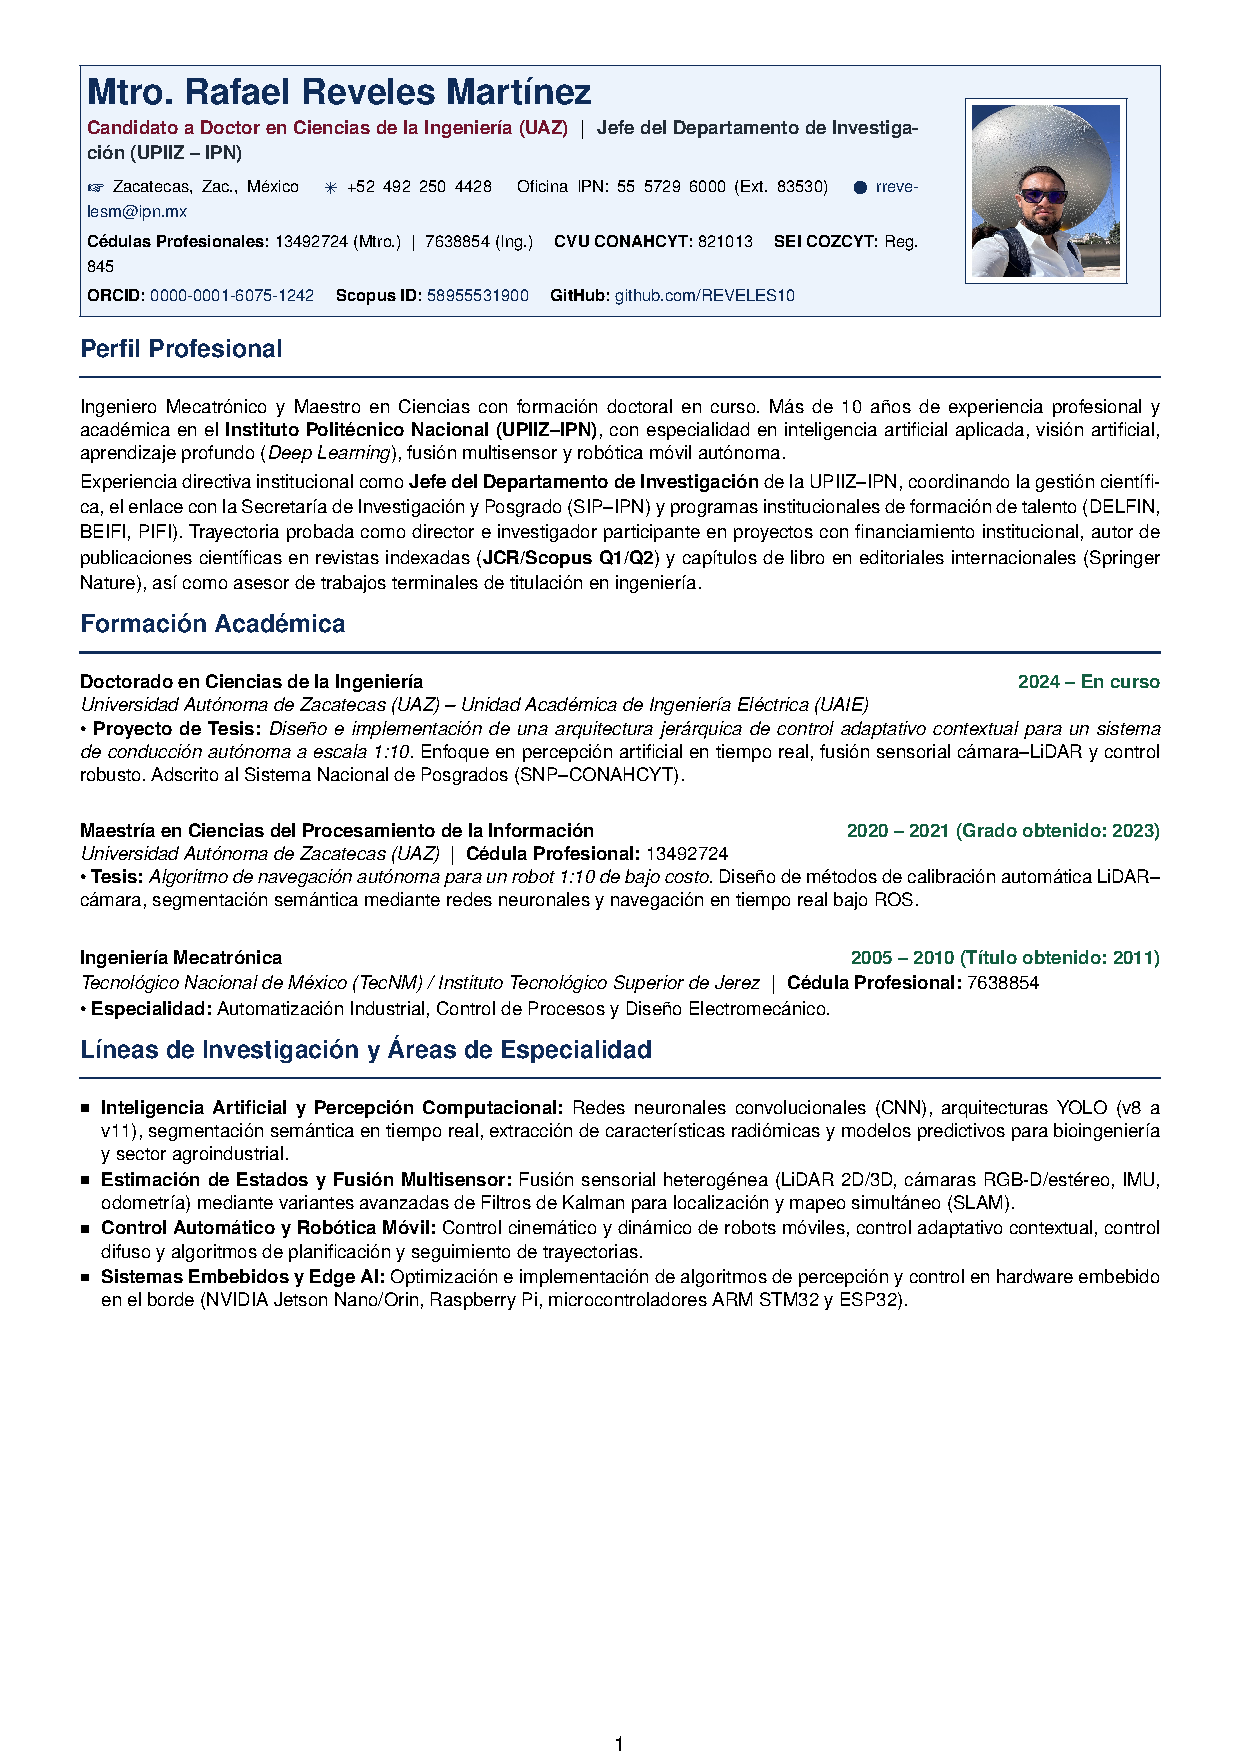
\includepdf[pages=1-2,pagecommand={\thispagestyle{empty}}]{anexos/cv_rafa.pdf}%
}{%
    \begin{center}
        \fbox{\parbox{0.88\textwidth}{%
            \centering\vspace{0.8em}
            \textbf{[Espacio para CV Resumido del Primer Asesor: \asesorANombre]}\\[0.4em]
            \small Deposite el archivo PDF en \texttt{anexos/cv-asesor-1.pdf} (máximo 2 páginas indicando cédula profesional).\\[0.8em]
        }}
    \end{center}
    \vspace{0.8cm}
}

\ifcsvoid{asesorBNombre}{}{%
    \IfFileExists{anexos/cv_sergio.pdf}{%
        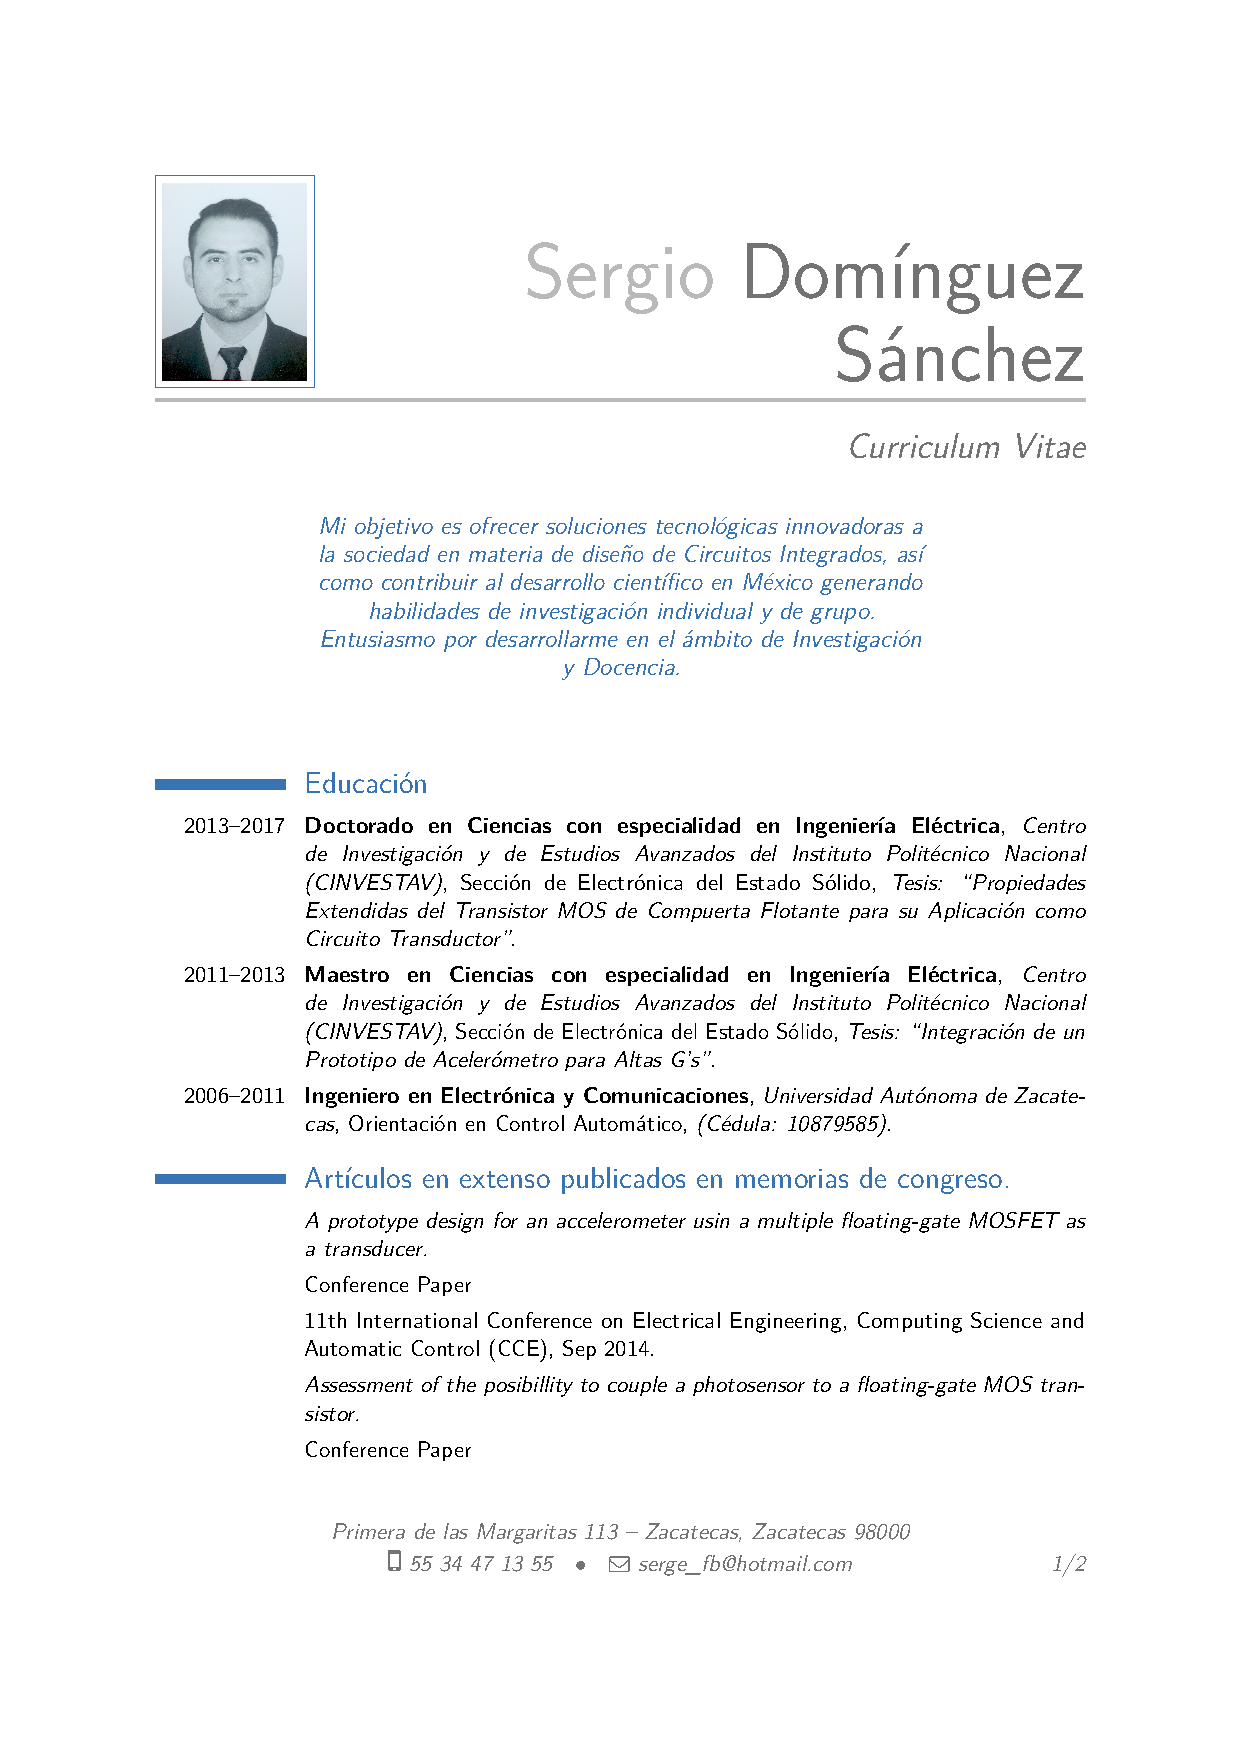
\includepdf[pages=1-2,pagecommand={\thispagestyle{empty}}]{anexos/cv_sergio.pdf}%
    }{%
        \begin{center}
            \fbox{\parbox{0.88\textwidth}{%
                \centering\vspace{0.8em}
                \textbf{[Espacio para CV Resumido del Segundo Asesor: \asesorBNombre]}\\[0.4em]
                \small Deposite el archivo PDF en \texttt{anexos/cv-asesor-2.pdf} (máximo 2 páginas indicando cédula profesional).\\[0.8em]
            }}
        \end{center}
        \vspace{0.8cm}
    }%
}

\ifcsvoid{asesorCNombre}{}{%
    \IfFileExists{anexos/cv_tala.pdf}{%
            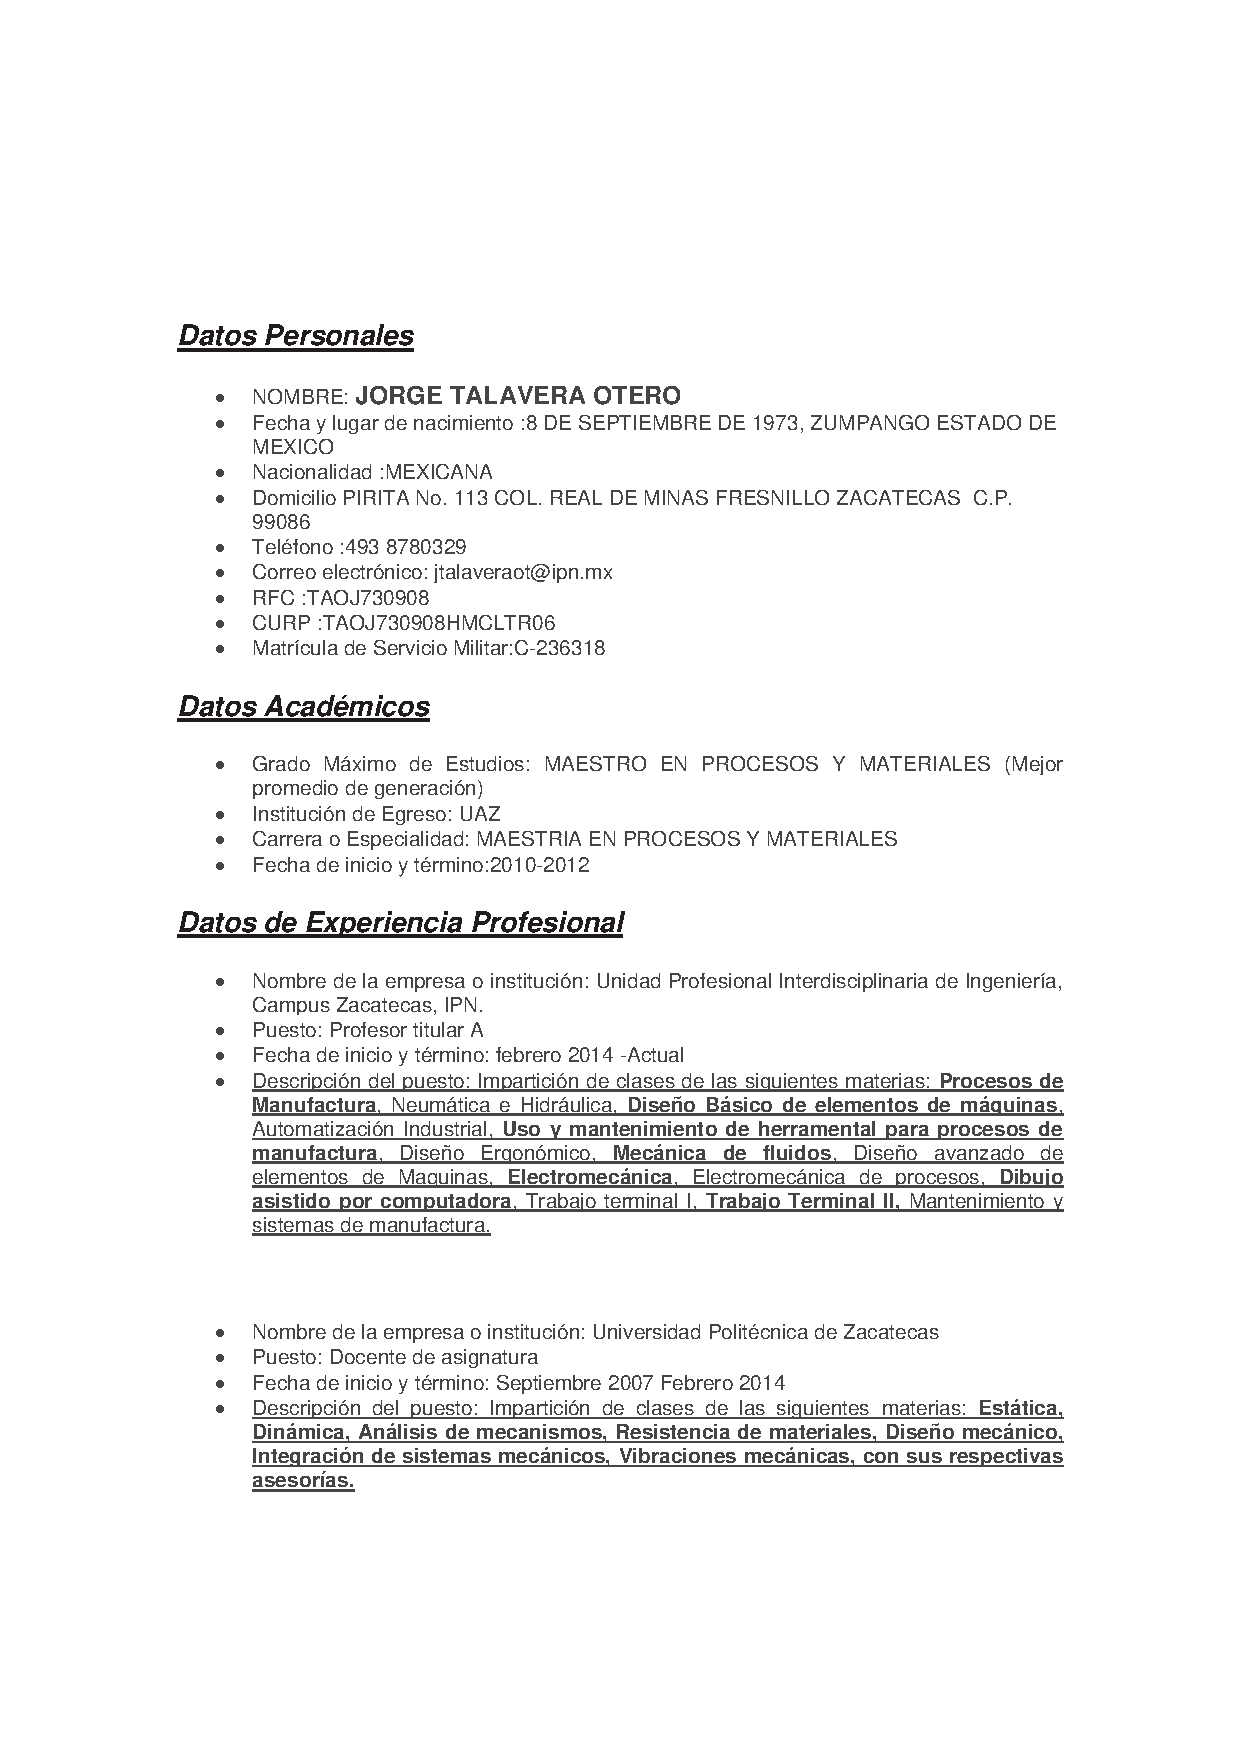
\includepdf[pages=1-2,pagecommand={\thispagestyle{empty}}]{anexos/cv_tala.pdf}%
    }{%
        \begin{center}
            \fbox{\parbox{0.88\textwidth}{%
                \centering\vspace{0.8em}
                \textbf{[Espacio para CV Resumido del Tercer Asesor: \asesorCNombre]}\\[0.4em]
                \small Deposite el archivo PDF en \texttt{anexos/cv-asesor-3.pdf} (máximo 2 páginas indicando cédula profesional).\\[0.8em]
            }}
        \end{center}
        \vspace{0.8cm}
    }%
}

% ------------------------------------------------------------------------------
% ÚLTIMA HOJA INSTITUCIONAL: ANEXO 2 (INSTRUMENTO DE EVALUACIÓN DE PROTOCOLO)
% ------------------------------------------------------------------------------
% El punto 18 del Anexo 1 establece que la última hoja del protocolo corresponderá
% al Anexo 2 del Reglamento para la evaluación de la Comisión Evaluadora.
% Coloque el archivo en "anexos/anexo-2-evaluacion.pdf" para su inclusión automática.

\IfFileExists{anexos/anexo_2.pdf}{%
    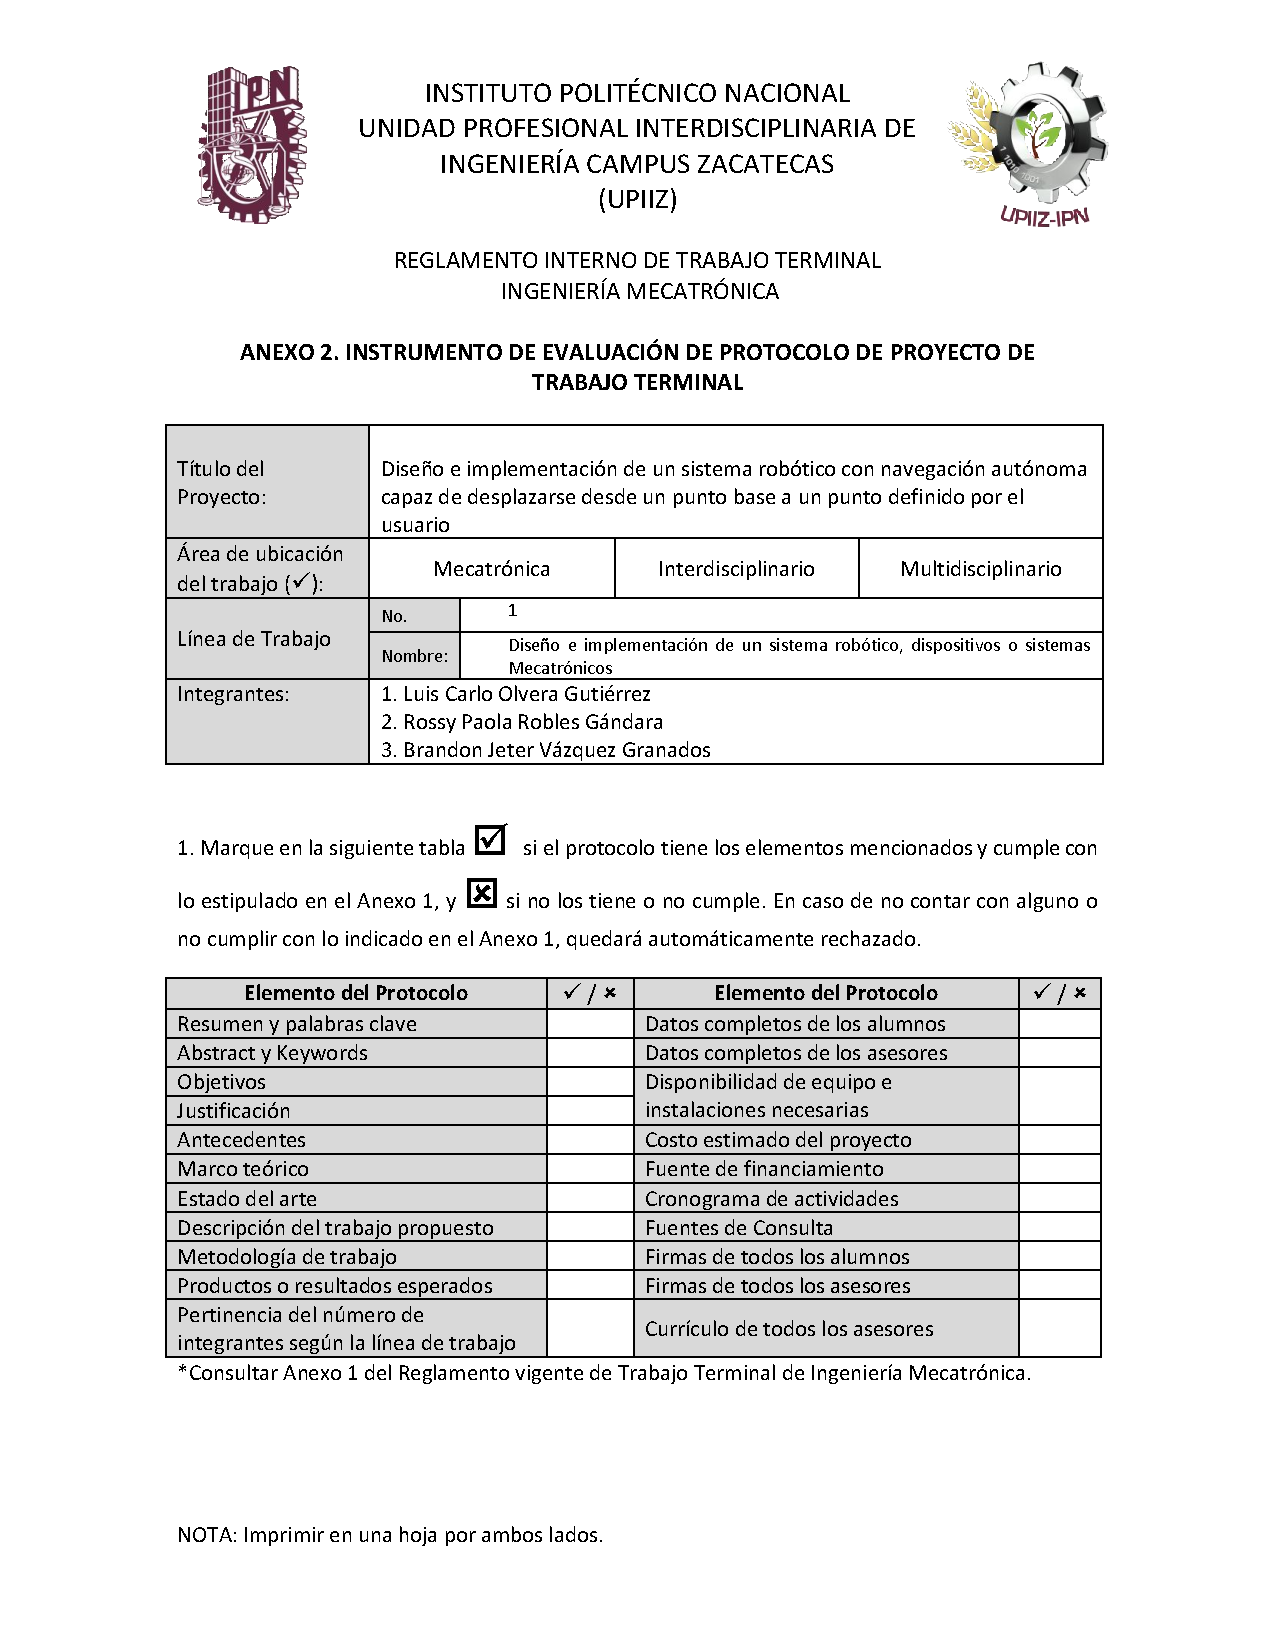
\includepdf[pages=1-3,pagecommand={\thispagestyle{empty}}]{anexos/anexo_2.pdf}%
}{%
    \vfill
    \begin{center}
        \fbox{\parbox{0.88\textwidth}{%
            \centering\vspace{0.8em}
            \textbf{[Última Hoja Institucional: Anexo 2 - Instrumento de Evaluación de Protocolo]}\\[0.4em]
            \small Para la entrega final, incorpore el formato oficial en \texttt{anexos/anexo-2-evaluacion.pdf} para que se anexe como la última hoja de acuerdo con el punto 18 del Anexo 1.\\[0.8em]
        }}
    \end{center}
    \vfill
}


\else
    % ==========================================================================
    % ESTRUCTURA DE REPORTE TÉCNICO (TRABAJO TERMINAL I Y TRABAJO TERMINAL II)
    % ==========================================================================
    % ==============================================================================
% Plantilla Institucional de Trabajo Terminal — UPIIZ IPN
% Archivo: capitulos/01-introduccion.tex
% ==============================================================================

\chapter{Introducción}
\label{cap:introduccion}

% ==============================================================================
% REGLA INSTITUCIONAL:
% A partir de esta sección inicia la numeración de páginas en números arábigos (1, 2, 3...).
%
% INSTRUCCIONES PEDAGÓGICAS:
% La introducción debe contextualizar el proyecto, describir la motivación y el
% alcance general del trabajo mecatrónico desarrollado, así como presentar un
% resumen estructurado del contenido de los capítulos que componen el documento.
% ==============================================================================

% Escriba aquí la descripción general y contextualización de su proyecto...
El presente Trabajo Terminal aborda el diseño y desarrollo de una solución mecatrónica orientada a resolver las necesidades identificadas en el ámbito de la ingeniería aplicada. En este documento se presentan de manera secuencial los fundamentos teóricos, metodológicos y de ingeniería que sustentan el proyecto.

A continuación se detalla la estructura capitular del reporte:
\begin{itemize}
    \item El \capref{cap:justificacion} expone la justificación técnica, social y económica del proyecto.
    \item El \capref{cap:antecedentes} presenta los antecedentes y trabajos previos relacionados.
    \item El \capref{cap:marco-teorico} sintetiza los fundamentos teóricos y modelos físico-matemáticos empleados.
    \item El \capref{cap:estado-del-arte} revisa el estado del arte y las tecnologías vigentes afines.
    \item El \capref{cap:planteamiento} define el planteamiento del problema y la solución propuesta.
    \item El \capref{cap:desarrollo} describe el desarrollo técnico detallado de la ingeniería mecatrónica.
    \item El \capref{cap:validacion} presenta el análisis y validación conforme a las especificaciones planteadas.
    \item El \capref{cap:conclusiones} establece las conclusiones derivadas del cumplimiento de los objetivos.
    \ifTTII
    \item El \capref{cap:trabajo-futuro} plantea las líneas de trabajo a futuro e iteraciones posteriores.
    \fi
\end{itemize}

% ==============================================================================
% OBJETIVOS DEL PROYECTO
% Copie aquí los objetivos EXACTAMENTE como fueron aprobados en el protocolo registrado.
% NO los modifique ni parafrasee sin aprobación formal del comité evaluador.
% ==============================================================================

\section{Objetivo general}
\label{sec:obj-general}

% Escriba aquí el objetivo general aprobado en el protocolo...
Desarrollar un sistema mecatrónico integral para la automatización y control del proceso definido, mediante el diseño e integración de subsistemas mecánicos, electrónicos y de software, a fin de validar su rendimiento ante especificaciones operativas cuantitativas.

\section{Objetivos específicos}
\label{sec:obj-especificos}

% Escriba aquí la lista de objetivos específicos aprobados en el protocolo...
\begin{enumerate}
    \item Establecer la lista de requerimientos y especificaciones de diseño mecatrónico a partir de las condiciones de operación.
    \item Diseñar y modelar los componentes mecánicos, estructurales y cinemáticos requeridos por el sistema.
    \item Diseñar y seleccionar la instrumentación electrónica, sensores, actuadores y etapas de potencia.
    \item Desarrollar los algoritmos de control, lógica de programación e interfaz de usuario para el sistema embebido.
    \item Evaluar y validar cuantitativamente el desempeño global del sistema mediante pruebas experimentales y análisis de error.
\end{enumerate}

    % ==============================================================================
% Plantilla Institucional de Trabajo Terminal — UPIIZ IPN
% Archivo: capitulos/02-justificacion.tex
% ==============================================================================
% LÍMITE INSTITUCIONAL: Máximo 1 página.
% ==============================================================================

\chapter{Justificación}
\label{cap:justificacion}

La investigación y desarrollo en sistemas vehiculares autónomos y asistidos demanda entornos de experimentación seguros, accesibles y altamente reproducibles. La experimentación directa sobre vehículos de tamaño real conlleva elevados costos de instrumentación, requerimientos de infraestructura especializada y riesgos considerables para la integridad física de los operadores e investigadores. En este contexto, el uso de plataformas mecatrónicas a escala 1:10 constituye una alternativa técnica idónea para la validación rigurosa de algoritmos de control, estimación de estados y procesamiento digital en tiempo real.

Desde la perspectiva técnica, el control de la velocidad longitudinal y del ángulo de dirección involucra dinámicas electromecánicas acopladas, no linealidades inherentes a la tracción y efectos de fricción e inercia variables. La formulación del sistema en espacio de estados proporciona un marco analítico robusto que permite no solo sintetizar leyes de control multivariable con especificaciones dinámicas estrictas (tiempo de establecimiento, sobrepaso y error en régimen permanente), sino también evaluar formalmente la controlabilidad y observabilidad del sistema y estimar variables no medibles directamente mediante observadores o filtros digitales.

Institucionalmente, el presente proyecto se encuentra plenamente alineado con la \textbf{Línea de investigación IV: Diseño e implementación de sistemas o técnicas de control} del Programa Académico de Ingeniería Mecatrónica de la UPIIZ-IPN. Si bien el énfasis principal radica en la teoría y aplicación de control moderno, el proyecto exige la integración sinérgica de las cuatro áreas de la disciplina: el análisis cinemático y geométrico del chasis (Mecánica), el diseño de etapas de potencia y acondicionamiento sensorial (Electrónica), el modelado y síntesis de la ley de control (Control) y el desarrollo de firmware embebido determinista (Programación).

Socialmente, el proyecto aporta una metodología transferible para el diseño de bancos de prueba docentes y de investigación en el Instituto Politécnico Nacional, facilitando la formación práctica de ingenieros en el desarrollo de tecnologías de movilidad terrestre y sistemas de transporte inteligente.

    % ==============================================================================
% Plantilla Institucional de Trabajo Terminal — UPIIZ IPN
% Archivo: capitulos/03-antecedentes.tex
% ==============================================================================
% LÍMITE NORMATIVO INSTITUCIONAL: 1 cuartilla (aproximadamente 1 página).
% ==============================================================================

\chapter{Antecedentes}
\label{cap:antecedentes}

En este capítulo se expone el contexto histórico y la evolución tecnológica previa del problema de estudio, identificando los antecedentes científicos directos y los proyectos desarrollados previamente a nivel internacional, nacional y dentro del Instituto Politécnico Nacional.

Se sugiere redactar este capítulo considerando las siguientes pautas:
\begin{itemize}
    \item \textbf{Evolución tecnológica del área:} Describa cómo han evolucionado históricamente los métodos, dispositivos y sistemas empleados para resolver la problemática planteada.
    \item \textbf{Trabajos previos en la UPIIZ-IPN:} Mencione si existen Trabajos Terminales, proyectos de investigación o bancos de laboratorio desarrollados previamente en la academia que sirvan como punto de partida o referencia directa para esta propuesta.
    \item \textbf{Limitaciones de los desarrollos previos:} Explique claramente qué aspectos no fueron cubiertos o qué áreas de oportunidad motivan el presente Trabajo Terminal (por ejemplo: falta de lazo cerrado, procesamiento en tiempo real limitado, requerimientos de portabilidad o costo excesivo).
\end{itemize}

\noindent La redacción debe mantenerse en pasado para investigaciones y proyectos concluidos, y en presente para el estado actual de los hechos.

    % ==============================================================================
% Plantilla Institucional de Trabajo Terminal — UPIIZ IPN
% Archivo: capitulos/04-marco-teorico.tex
% ==============================================================================
% LÍMITE NORMATIVO INSTITUCIONAL: Máximo 3 páginas.
% ==============================================================================

\chapter{Marco Teórico}
\label{cap:marco-teorico}

En este capítulo se presentan los fundamentos físico-matemáticos indispensables que sustentan el modelado dinámico, el análisis de estabilidad, las leyes de control y las técnicas de procesamiento empleadas en el proyecto \cite{ogata2010modern}.

% ------------------------------------------------------------------------------
\section{Modelado físico-matemático del sistema}
\label{sec:marco-modelado}

Describa las ecuaciones diferenciales que gobiernan el comportamiento del sistema mecatrónico. Por ejemplo, para un sistema electromecánico lineal invariante en el tiempo continuo, la representación general en espacio de estados se formula como:
\begin{align}
    \dot{\mathbf{x}}(t) &= \mathbf{A}\mathbf{x}(t) + \mathbf{B}\mathbf{u}(t) \label{eq:espacio-estados-continuo} \\
    \mathbf{y}(t) &= \mathbf{C}\mathbf{x}(t) + \mathbf{D}\mathbf{u}(t) \label{eq:salida-continuo}
\end{align}
donde $\mathbf{x}(t) \in \mathbb{R}^n$ es el vector de variables de estado, $\mathbf{u}(t) \in \mathbb{R}^m$ es el vector de entradas de control, $\mathbf{y}(t) \in \mathbb{R}^p$ es el vector de salidas medidas, y $\mathbf{A}, \mathbf{B}, \mathbf{C}, \mathbf{D}$ son las matrices del sistema.

% ------------------------------------------------------------------------------
\section{Análisis de controlabilidad y leyes de control}
\label{sec:marco-control}

La controlabilidad del sistema garantiza que es posible transferir el estado del sistema desde cualquier condición inicial hasta el origen en tiempo finito mediante una ley de control admisible. La matriz de controlabilidad $\mathcal{C}$ se define como:
\begin{equation}
    \mathcal{C} = \begin{bmatrix} \mathbf{B} & \mathbf{A}\mathbf{B} & \mathbf{A}^2\mathbf{B} & \cdots & \mathbf{A}^{n-1}\mathbf{B} \end{bmatrix}, \quad \text{rank}(\mathcal{C}) = n
    \label{eq:matriz-controlabilidad-marco}
\end{equation}

La ley de control por realimentación de estados con precompensación para seguimiento de referencias $\mathbf{r}(t)$ se expresa mediante:
\begin{equation}
    \mathbf{u}(t) = -\mathbf{K}\mathbf{x}(t) + \mathbf{N}\mathbf{r}(t)
    \label{eq:ley-control-marco}
\end{equation}
donde $\mathbf{K}$ representa la matriz de ganancias calculada para satisfacer las especificaciones dinámicas de tiempo de establecimiento y sobrepaso porcentual.

Recuerde expresar todas las magnitudes físicas utilizando el paquete \texttt{siunitx}, por ejemplo: tensión de \qty{12.0}{\volt}, corriente de \qty{2.5}{\ampere}, frecuencia de muestreo de \qty{1.0}{\kilo\hertz} y par motor de \qty{0.45}{\newton\meter}.

    % ==============================================================================
% Plantilla Institucional de Trabajo Terminal — UPIIZ IPN
% Archivo: capitulos/05-estado-del-arte.tex
% ==============================================================================

\chapter{Estado del arte}
\label{cap:estado-del-arte}

% ==============================================================================
% REQUISITO INSTITUCIONAL:
% Extensión: Máximo CUATRO páginas.
%
% INSTRUCCIONES PEDAGÓGICAS:
% Realice una revisión crítica y comparativa de las tecnologías, productos comerciales,
% patentes y publicaciones científicas recientes (últimos 5 años preferentemente)
% relacionadas directamente con el problema que resuelve su proyecto.
%
% No se limite a listar artículos; elabore un análisis comparativo destacando:
% - Ventajas y desventajas de cada enfoque existente.
% - Parámetros de desempeño, costos, complejidad y limitaciones.
% - La brecha tecnológica u oportunidad que justifica la solución propuesta en este TT.
% ==============================================================================

\section{Tecnologías y soluciones existentes}
\label{sec:arte-tecnologias}

% Escriba aquí la revisión de soluciones comerciales y académicas...
En el ámbito internacional, el desarrollo de soluciones mecatrónicas para este tipo de aplicaciones ha experimentado un crecimiento notable impulsado por avances en microelectrónica y algoritmos de optimización. Diversos autores han propuesto arquitecturas basadas en controladores lógicos programables, microcontroladores de 32 bits y computadoras de placa reducida (SBC) \cite{ogata2010modern, arizona2023embedded}.

Asimismo, en la literatura especializada se reportan implementaciones con diferentes grados de autonomía y precisión, empleando esquemas de comunicación inalámbrica y protocolos industriales \cite{smith2022control, ieee2021robotics}.

\section{Comparativa técnica de enfoques}
\label{sec:arte-comparativa}

A fin de situar la presente propuesta frente a las alternativas documentadas, la \tabref{tab:comparativa-arte} resume las principales características operativas de las tecnologías analizadas.

\begin{table}[htbp]
    \centering
    \caption{Comparación técnica de tecnologías y enfoques existentes.}
    \label{tab:comparativa-arte}
    \begin{tabularx}{\textwidth}{p{3.0cm} X X p{3.2cm}}
        \toprule
        \textbf{Enfoque / Solución} & \textbf{Ventajas} & \textbf{Desventajas} & \textbf{Aplicabilidad en este TT} \\
        \midrule
        Sistemas comerciales propietarios & Alta robustez y soporte de fábrica & Costo elevado y nula personalización & Limitada para fines académicos \\
        Plataformas abiertas modulares & Bajo costo y alta flexibilidad & Mayor complejidad de integración & Base fundamental de este trabajo \\
        Control clásico analógico & Simplicidad circuital & Sensibilidad a ruido y deriva térmica & Superado por control digital \\
        \bottomrule
    \end{tabularx}
\end{table}

\section{Oportunidad y aportación de la propuesta}
\label{sec:arte-oportunidad}

A partir de la revisión realizada, se identifica una oportunidad de desarrollo enfocada en optimizar la relación costo-rendimiento mediante la integración de hardware de procesamiento accesible y técnicas de control robustas adaptadas a las condiciones operativas locales.

    % ==============================================================================
% Plantilla Institucional de Trabajo Terminal — UPIIZ IPN
% Archivo: capitulos/06-planteamiento-problema.tex
% ==============================================================================

\chapter{Planteamiento del Problema}
\label{cap:planteamiento}

En este capítulo se define de manera formal y precisa la problemática de ingeniería que motiva el Trabajo Terminal, las restricciones operativas del sistema y la solución mecatrónica interdisciplinaria propuesta.

% ------------------------------------------------------------------------------
\section{Formulación del problema de ingeniería}
\label{sec:planteamiento-problema}

Redacte de forma clara los síntomas y causas de la problemática que se pretende resolver. Identifique las limitaciones que presentan los sistemas actuales y formule la necesidad concreta de diseño o automatización:
\begin{enumerate}
    \item \textbf{Deficiencia o limitación principal:} Describa qué fenómeno físico, ineficiencia de proceso o restricción operacional impide alcanzar el desempeño óptimo.
    \item \textbf{Causas técnicas identificadas:} Explique los factores electromecánicos, perturbaciones ambientales o carencias sensoriales asociadas.
    \item \textbf{Consecuencias de no resolver el problema:} Puntualice los riesgos de falla, pérdidas económicas o desviaciones de calidad.
\end{enumerate}

% ------------------------------------------------------------------------------
\section{Solución mecatrónica propuesta}
\label{sec:solucion-propuesta}

Exponga la propuesta técnica de solución, detallando explícitamente cómo participará cada una de las cuatro áreas de la Ingeniería Mecatrónica:
\begin{itemize}
    \item \textbf{Mecánica:} Diseño del mecanismo, análisis cinemático y dinámico, cálculo de esfuerzos estructurales y modelado CAD 3D de piezas y ensambles.
    \item \textbf{Electrónica:} Selección y acondicionamiento de sensores, diseño de etapas de potencia, aislamiento galvánico y gestión eficiente de la energía.
    \item \textbf{Control:} Formulación de modelos dinámicos, diseño de observadores/estimadores y síntesis de leyes de control en lazo cerrado para garantizar estabilidad y seguimiento.
    \item \textbf{Programación:} Implementación de firmware determinista en tiempo real, comunicación por buses industriales/digitales e interfaz de supervisión telemática.
\end{itemize}

    % ==============================================================================
% Plantilla Institucional de Trabajo Terminal — UPIIZ IPN
% Archivo: capitulos/07-desarrollo.tex
% ==============================================================================

\chapter{Desarrollo del Sistema Mecatrónico}
\label{cap:desarrollo}

En este capítulo se expone la metodología técnica de desarrollo, la arquitectura funcional de los subsistemas, la matriz de especificaciones de diseño y el proceso de integración mecatrónica del prototipo.

% ------------------------------------------------------------------------------
\section{Arquitectura funcional y flujo de información}
\label{sec:desarrollo-arquitectura}

Describa la estructura en bloques del sistema y el flujo secuencial de señales y energía entre subsistemas:
\begin{enumerate}
    \item \textbf{Etapa de Sensado y Adquisición:} Instrumentación y captura periódica de variables físicas del proceso.
    \item \textbf{Etapa de Filtrado y Procesamiento:} Algoritmos digitales de acondicionamiento de señales y estimación de estados.
    \item \textbf{Etapa de Control y Algoritmos:} Evaluación en tiempo real de la ley de control en lazo cerrado ($f_s \ge \qty{1.0}{\kilo\hertz}$).
    \item \textbf{Etapa de Actuación y Potencia:} Modulación de señales de control hacia los actuadores electromecánicos.
    \item \textbf{Etapa de Supervisión y Comunicación:} Transmisión telemática de datos hacia la estación de monitoreo.
\end{enumerate}

% ------------------------------------------------------------------------------
\section{Matriz de requerimientos y especificaciones cuantitativas}
\label{sec:desarrollo-especificaciones}

En la \tabref{tab:especificaciones-diseno} se presentan las especificaciones cuantitativas de desempeño objetivo fijadas para el proyecto.

\begin{table}[htbp]
    \centering
    \caption{Especificaciones cuantitativas de desempeño del sistema mecatrónico.}
    \label{tab:especificaciones-diseno}
    \begin{tabularx}{\textwidth}{p{6.5cm} c X}
        \toprule
        \textbf{Parámetro de Desempeño} & \textbf{Símbolo / Métrica} & \textbf{Valor Objetivo} \\
        \midrule
        Rango de operación principal & $y(t)$ & $\qty{0.0}{\meter}$ a $\qty{2.0}{\meter}$ \\
        Tiempo de establecimiento ($2\,\%$) & $t_s$ & $\le \qty{0.50}{\second}$ \\
        Sobrepaso porcentual máximo & $M_p$ & $\le 10\,\%$ \\
        Error en régimen permanente & $|e_{ss}|$ & $\le \qty{0.05}{\unit{\meter}}$ \\
        Frecuencia de muestreo del lazo digital & $f_s = 1/T_s$ & $\ge \qty{1.0}{\kilo\hertz}$ \\
        Masa total del prototipo integrado & $m_{\text{total}}$ & $\le \qty{5.0}{\kilo\gram}$ \\
        Tensión de alimentación nominal & $V_{\text{bat}}$ & $\qty{12.0}{\volt}$ \\
        \bottomrule
    \end{tabularx}
\end{table}

% ------------------------------------------------------------------------------
\section{Integración física y manufactura de subsistemas}
\label{sec:desarrollo-integracion}

Detalle los procesos de manufactura (impresión 3D, mecanizado CNC, corte láser, ensamble de circuitos impresos PCB) y las estrategias de acoplamiento físico empleadas para garantizar la rigidez y confiabilidad del prototipo.

    % ==============================================================================
% Plantilla Institucional de Trabajo Terminal — UPIIZ IPN
% Archivo: capitulos/08-validacion.tex
% ==============================================================================

\chapter{\tituloValidacion}
\label{cap:validacion}

En este capítulo se describen los protocolos experimentales planificados, las métricas cuantitativas que se utilizarán y los criterios de aceptación para evaluar el desempeño integral del robot rover en el entorno de pruebas de terreno irregular.

% ------------------------------------------------------------------------------
\section{Métricas cuantitativas de evaluación de la misión}
\label{sec:validacion-metricas-rover}

Para evaluar rigurosamente el desempeño de cada subsistema y la eficacia global de la misión de exploración, se emplearán las siguientes métricas:

\begin{enumerate}
    \item \textbf{Error de posición euclidiano en navegación sin GPS:}
    \begin{equation}
        e_p(t) = \sqrt{\big(x_r(t) - x(t)\big)^2 + \big(y_r(t) - y(t)\big)^2}
        \label{eq:error-posicion-rover}
    \end{equation}
    \item \textbf{Tasa de éxito en la detección de muestras geológicas ($\eta_{\text{det}}$):}
    \begin{equation}
        \eta_{\text{det}} = \frac{N_{\text{muestras detectadas}}}{N_{\text{muestras presentes en el campo}}} \times 100\,\%
        \label{eq:tasa-deteccion}
    \end{equation}
    \item \textbf{Tasa de éxito del mecanismo de recolección ($\eta_{\text{rec}}$):}
    \begin{equation}
        \eta_{\text{rec}} = \frac{N_{\text{muestras recolectadas y aseguradas}}}{N_{\text{intentos de recolección}}} \times 100\,\%
        \label{eq:tasa-recoleccion}
    \end{equation}
    \item \textbf{Eficiencia global de cumplimiento de misión ($\eta_{\text{misión}}$):}
    \begin{equation}
        \eta_{\text{misión}} = \frac{N_{\text{misiones completadas exitosamente}}}{N_{\text{misiones ejecutadas}}} \times 100\,\%
        \label{eq:eficiencia-mision}
    \end{equation}
\end{enumerate}

% ------------------------------------------------------------------------------
\section{Protocolo y criterios de validación experimental en pista}
\label{sec:validacion-protocolo-rover}

En la \tabref{tab:comparativa-validacion} se resumen los criterios de aceptación cuantitativos que se verificarán durante los ensayos de campo en el escenario experimental de terreno irregular.

\begin{table}[htbp]
    \centering
    \caption{Criterios de validación y especificaciones de desempeño por verificar en el rover.}
    \label{tab:comparativa-validacion}
    \begin{tabularx}{\textwidth}{p{3.8cm} c p{3.8cm} X}
        \toprule
        \textbf{Prueba / Subsistema} & \textbf{Especificación} & \textbf{Método de Medición} & \textbf{Criterio de Aceptación} \\
        \midrule
        Movilidad en pendiente & $\ge \ang{15}$ de inclinación & Ensayos en rampa de tierra & Ascenso sin deslizamiento crítico \\
        Localización sin GPS & $e_p \le 5\,\%$ de trayecto & Contraste con marcas terrestres & Deriva acotada en circuito \\
        Detección visual de muestras & $\eta_{\text{det}} \ge 85\,\%$ & Registro de cámara y HMI & Reconocimiento a $\ge \qty{1.0}{\meter}$ \\
        Recolección y depósito & $\eta_{\text{rec}} \ge 80\,\%$ & Ensayos de manipulación & Captura, traslado y descarga \\
        Misión autónoma integral & $\eta_{\text{misión}} \ge 75\,\%$ & Ejecución completa sin GPS & Retorno exitoso a zona base \\
        \bottomrule
    \end{tabularx}
\end{table}

El cumplimiento de estos criterios permitirá demostrar la viabilidad, robustez y autonomía de la plataforma robótica desarrollada para misiones de exploración terrestre y lunar análoga.

    % ==============================================================================
% Plantilla Institucional de Trabajo Terminal — UPIIZ IPN
% Archivo: capitulos/09-conclusiones.tex
% ==============================================================================

\chapter{Resultados Esperados y Conclusiones del Protocolo}
\label{cap:conclusiones}

Con base en la formulación analítica, el plan de trabajo propuesto y la articulación sinérgica de las cuatro áreas de la ingeniería mecatrónica, se proyecta alcanzar los siguientes resultados y contribuciones al concluir las etapas de Trabajo Terminal I y II:

\begin{enumerate}
    \item \textbf{Proyección respecto al Objetivo Específico 1:} Se obtendrá una representación dinámica continua y discreta en espacio de estados que modele con fidelidad el comportamiento acoplado del tren de tracción y del mecanismo de dirección Ackermann, sustentada en la identificación paramétrica experimental de los componentes electromecánicos.
    \item \textbf{Proyección respecto al Objetivo Específico 2:} Se demostrará la controlabilidad y observabilidad del sistema mecatrónico, sintetizando la matriz de ganancias de realimentación $\mathbf{K}$ que garantizará una respuesta transitoria rápida ($t_s \le \qty{0.50}{\second}$) con un sobrepaso controlado ($M_p \le 10\,\%$) y sin saturación excesiva de las etapas de potencia.
    \item \textbf{Proyección respecto al Objetivo Específico 3:} Se consolidará una plataforma vehicular a escala 1:10 instrumentada, modular y reproducible, con electrónica de potencia aislada y firmware determinista en lenguaje C++ ejecutado a \qty{1}{\kilo\hertz} sobre un microcontrolador de 32 bits.
    \item \textbf{Proyección respecto al Objetivo Específico 4:} Se establecerá un protocolo de validación experimental cuantificable que permitirá verificar en pista el cumplimiento de los márgenes de error especificados ($\text{MAE}_v \le \qty{0.05}{\meter\per\second}$, $\text{RMSE}_v \le \qty{0.08}{\meter\per\second}$), evaluando la capacidad de rechazo ante perturbaciones y la robustez del sistema ante caídas de tensión de la batería.
\end{enumerate}

En conclusión, la ejecución del proyecto bajo los lineamientos de la Línea IV de la UPIIZ-IPN proporcionará un banco de pruebas mecatrónico de alto valor académico, sirviendo de base experimental sólida para futuras investigaciones en sistemas de control y vehículos inteligentes.


    % Trabajo a Futuro (EXCLUSIVO para TT II / Reporte Final)
    \ifTTII
        % ==============================================================================
% Plantilla Institucional de Trabajo Terminal — UPIIZ IPN
% Archivo: capitulos/10-trabajo-futuro.tex
% ==============================================================================
% NOTA: Este capítulo se incluye condicionalmente solo para TT II.
% En PROTOCOLO y TT I se omite automáticamente.
% ==============================================================================

\chapter{Trabajo Futuro}
\label{cap:trabajo-futuro}

En este capítulo se proponen las líneas de investigación, mejoras de diseño y extensiones tecnológicas recomendadas para dar continuidad al proyecto desarrollado:

\begin{enumerate}
    \item \textbf{Optimizaciones mecánicas y estructurales:} Rediseño de componentes para reducción de masa, selección de materiales avanzados o incorporación de mecanismos con mayor grado de libertad.
    \item \textbf{Mejoras en sensado y electrónica:} Incorporación de sensores de mayor resolución, implementación de etapas de potencia más eficientes o integración de buses de comunicación industrial.
    \item \textbf{Evolución de algoritmos y control:} Exploración de técnicas de control adaptativo, predictivo basado en modelos (MPC) o algoritmos de aprendizaje por refuerzo.
    \item \textbf{Escalabilidad y aplicaciones industriales:} Adaptación del prototipo para pruebas en entornos productivos reales o integración con plataformas de Internet de las Cosas (IoT) e Industria 4.0.
\end{enumerate}

    \fi

    % Bibliografía en formato IEEE
    \clearpage
    \addcontentsline{toc}{chapter}{Bibliografía}
    \bibliographystyle{IEEEtran}
    \bibliography{bibliografia/referencias}

    % Apéndices
    \clearpage
    % ==============================================================================
% Plantilla Institucional de Trabajo Terminal — UPIIZ IPN
% Archivo: apendices/apendices.tex
% ==============================================================================
% Configuración y contenido de los Apéndices de ingeniería del proyecto.
% ==============================================================================

\appendix

% ==============================================================================
% APÉNDICE A: CÁLCULOS DETALLADOS Y SELECCIÓN DE COMPONENTES
% ==============================================================================
\chapter{Cálculos detallados de ingeniería}
\label{ap:calculos}

% Incluya aquí desarrollos matemáticos extensos, demostraciones o cálculos de dimensionamiento...
En este apéndice se detallan los cálculos de dimensionamiento mecánico y térmico.

\section{Cálculo del par motor requerido}
Para una masa total $m = \qty{3.5}{\kilo\gram}$ y un radio de rueda $r = \qty{0.05}{\meter}$, considerando una aceleración angular $\alpha = \qty{4.0}{\radian\per\second\squared}$ y una pendiente máxima $\theta = \ang{15}$, el par estático y dinámico se calcula como:

\begin{equation}
    \tau_{\text{total}} = (m \, g \, \sin\theta + m \, a) \cdot r + I \cdot \alpha
    \label{eq:par-calculo}
\end{equation}

\noindent Sustituyendo los valores numéricos correspondientes:
\begin{equation}
    \tau_{\text{total}} = (3.5 \cdot 9.81 \cdot \sin(\ang{15}) + 3.5 \cdot 0.2) \cdot 0.05 \approx \qty{0.479}{\newton\meter}
\end{equation}

% ==============================================================================
% APÉNDICE B: PLANOS MECÁNICOS Y VISTAS DE ENSAMBLE
% ==============================================================================
\chapter{Planos mecánicos y de ensamble}
\label{ap:planos}

% Incluya aquí planos normalizados, vistas de ensamble y despiece...
En este apartado se incorporan los planos de manufactura normalizados con cotas, tolerancias dimensionales y acabados superficiales requeridos para la fabricación de los componentes estructurales.

\begin{figure}[htbp]
    \centering
    \fbox{\parbox[c][6cm][c]{0.85\textwidth}{\centering\textbf{[Espacio reservado para Plano de Ensamble / Vista en Explosión]}\\
    \small Inserte aquí el plano en formato PDF o imagen vectorial (\texttt{\textbackslash includegraphics[width=0.9\textbackslash textwidth]\{...\}})}}
    \caption{Plano de ensamble general del sistema mecatrónico.}
    \label{fig:plano-ensamble}
\end{figure}

% ==============================================================================
% APÉNDICE C: DIAGRAMAS ELECTRÓNICOS Y ESQUEMÁTICOS
% ==============================================================================
\chapter{Diagramas esquemáticos y ruteo de PCB}
\label{ap:esquematicos}

% Incluya aquí diagramas de conexiones, circuitos impresos y distribución de terminales...
En la \figref{fig:diagrama-conexiones} se presenta la topología de interconexión entre la unidad de procesamiento, los sensores y las etapas de potencia.

\begin{figure}[htbp]
    \centering
    \fbox{\parbox[c][5cm][c]{0.85\textwidth}{\centering\textbf{[Espacio reservado para Diagrama Esquemático Electrónico]}\\
    \small Inserte aquí el diagrama esquemático exportado desde KiCAD, Altium o Eagle}}
    \caption{Diagrama esquemático de la etapa de potencia e instrumentación.}
    \label{fig:diagrama-conexiones}
\end{figure}


    % Cronograma de TT II (EXCLUSIVO para el Reporte de TT I)
    \ifTTI
        % ==============================================================================
% Plantilla Institucional de Trabajo Terminal — UPIIZ IPN
% Archivo: apendices/cronograma-tt2.tex
% ==============================================================================
% Cronograma detallado de actividades para Trabajo Terminal II.
% ==============================================================================

\chapter{Cronograma de Actividades para Trabajo Terminal II}
\label{ap:cronograma-tt2}

En el presente apéndice se detalla la planeación temporal de las fases de manufactura, implementación, pruebas unitarias, integración mecatrónica y validación experimental que se llevarán a cabo en la asignatura de Trabajo Terminal II para culminar el proyecto.

\begin{table}[htbp]
    \centering
    \caption{Cronograma general de actividades y entregables para Trabajo Terminal II.}
    \label{tab:cronograma-tt2}
    \begin{tabularx}{\textwidth}{p{4.8cm} c c c c X}
        \toprule
        \textbf{Fase / Actividad Planificada} & \textbf{Mes 1} & \textbf{Mes 2} & \textbf{Mes 3} & \textbf{Mes 4} & \textbf{Entregable / Evidencia} \\
        \midrule
        Fase 10: Manufactura e integración de hardware & $\blacksquare$ & & & & Estructura física y circuitos ensamblados \\
        Fase 11: Implementación de firmware y control & & $\blacksquare$ & & & Firmware operativo en tiempo real \\
        Fase 12: Pruebas unitarias de subsistemas & & $\blacksquare$ & $\blacksquare$ & & Reporte de caracterización sensorial \\
        Fase 13: Validación experimental en banco/pista & & & $\blacksquare$ & $\blacksquare$ & Registro de datos de pruebas (MAE, RMSE) \\
        Fase 14: Reporte final y preparación de defensa oral & & & & $\blacksquare$ & Documento final y prototipo validado \\
        \bottomrule
    \end{tabularx}
\end{table}

    \fi
\fi

\end{document}
